% % created on 2019-12-13
% % @author : bmazoyer

% % Lines to compile only this capter
% \documentclass[11pt, twoside, a4paper, openright]{report}
% \usepackage[utf8]{inputenc}
% \DeclareUnicodeCharacter{223C}{~}

%Bibliography style
% \usepackage[square, numbers]{natbib}
% \usepackage[round]{natbib}
% \usepackage{biblatex}
% \bibliographystyle{unsrtnat}
% \bibliographystyle{unsrt}
% \bibliographystyle{plain}
% \bibliographystyle{aa}
% \usepackage[backend=bibtex,style=authoryear,natbib=true]{biblatex} 
\usepackage[
backend=biber,
style=authoryear,
citestyle=authoryear,
url=false
]{biblatex}
\addbibresource{../source/library.bib}

\usepackage[T1]{fontenc}
\usepackage[french]{babel}
\usepackage{csquotes}  % used for citations (recommended when using biblatex)
%\usepackage{helvet}
%\renewcommand{\familydefault}{\sfdefault}
\usepackage{mathptmx}
\usepackage{amssymb}
\usepackage{geometry} 
\usepackage{xcolor}
\usepackage[absolute,overlay]{textpos}
\usepackage{graphicx}
\usepackage{lipsum}
\usepackage[explicit]{titlesec}
\usepackage{lmodern}
\usepackage{color}
\usepackage{array}
\usepackage{mathtools}
\usepackage{caption}
\usepackage{multicol}
\usepackage{booktabs}
\usepackage{enumitem}
\usepackage{hyperref}
\usepackage{afterpage}
\usepackage{emptypage}
\usepackage{setspace}
\usepackage{pgffor}
    \setlength{\columnseprule}{0pt}
    \setlength\columnsep{10pt}
\usepackage[francais,nohints]{minitoc}
    \setcounter{minitocdepth}{3}
 
 %https://la-bibliotex.fr/2019/02/03/ecrire-les-nombres-et-les-unites-avec-latex/   
\usepackage{siunitx}
% \sisetup{
%     detect-all,
%      output-decimal-marker={,},
%      group-minimum-digits = 3,
%      group-separator={~},
%      number-unit-separator={~},
%      inter-unit-product={~},
%      list-separator = {, },
%      list-final-separator = { et },
%      range-phrase = --,
%      separate-uncertainty = true,
%      multi-part-units = single,
%      list-units = single,
%      range-units = single
%     }
\usepackage{physics}
\usepackage{isotope}

\usepackage[perpage]{footmisc} % to reset the counter of footnote each page

    
\usepackage{fancyhdr}			% Entête et pieds de page. Doit être placé APRES geometry
\pagestyle{fancy}		% Indique que le style de la page sera justement fancy
%\lfoot[\thepage]{} 		% gauche du pied de page
%\cfoot{} 			% milieu du pied de page
%\rfoot[]{\thepage} 
\fancyfoot{} % vide le pied~de~page
\fancyfoot[LE,RO]{\thepage}
\fancyfoot[LO,CE]{}% droite du pied de page
\fancyhead{}	
\fancyhead[LE]{\leftmark}	
\fancyhead[RO]{\rightmark}

\fancypagestyle{plain}{%
\fancyhf{} % vide l’en-tête et le pied~de~page.
\fancyfoot[LE,RO]{\thepage} % numéro de la page en cours en gras% et centré en pied~de~page.
\renewcommand{\headrulewidth}{0pt}
\renewcommand{\footrulewidth}{0pt}}



% Premiere page des chapitres
\newlength\chapnumb
\setlength\chapnumb{3cm}
 
\titleformat{\chapter}[block] {
  \normalfont}{}{0pt} { %police
    \parbox[b]{\chapnumb}{
      \fontsize{120}{110}\selectfont\thechapter} %taille du chiffre
      \parbox[b]{\dimexpr\textwidth-\chapnumb\relax}{
        \raggedleft 
        \hfill{\bfseries\Huge#1}\\ %taille du titre
        \rule{\dimexpr\textwidth-\chapnumb\relax}{0.4pt} %ligne de separation
  }
}
 
 %premiere page chapitre non numerote (remerciement, table des matieres ...)
 
\titleformat{name=\chapter,numberless}[block]
{\normalfont}{}{0pt}
{   
    \parbox[b]{\dimexpr\textwidth}{%   
    \hfill{\bfseries\Huge#1}\\
  \rule{\dimexpr\textwidth}{0.4pt}}}
    
 %   \titleformat{name=\chapter,numberless}[block]
%{\normalfont}{}{0pt}
%{\parbox[b]{\chapnumb}{%
%   \mbox{}}%
%  \parbox[b]{\dimexpr\textwidth-\chapnumb\relax}{%
%    \raggedleft%
%    \hfill{\bfseries\Huge#1}\\
%    \rule{\dimexpr\textwidth-\chapnumb\relax}{0.4pt}}}


%%%    SIunitx
\sisetup{locale = FR,
  % inter-unit-product=\ensuremath{\cdot},
  inter-unit-product=\ensuremath{\,},
  per-mode=reciprocal,
  separate-uncertainty = true,
  detect-all
}
\DeclareSIUnit{\Mpc}{Mpc}
\DeclareSIUnit{\kpc}{kpc}
\DeclareSIUnit{\Gpc}{Gpc}
\DeclareSIUnit{\h}{\textit{h}~}
\DeclareSIUnit{\perh}{\textit{h}^{-1}\,}

%%% Geometry
\geometry{
left=20mm,
top=30mm,
right=20mm,
bottom=30mm
}

%%% Color
\definecolor{bordeau}{rgb}{0.3515625,0,0.234375}

%%% Commands
\newcommand{\Nmocks}{\num{30}}
\newcommand{\hMpc}{h^{-1}\,\mathrm{Mpc}}
\newcommand{\hGpc}{h^{-1}\,\mathrm{Gpc}}
\newcommand{\kms}{\mathrm{km\,s^{-1}}}

\newcommand{\lya}{Ly$\alpha$}
\newcommand{\lyb}{Ly$\beta$}
\newcommand{\lyalya}{Ly$\alpha$(Ly$\alpha$)}
\newcommand{\lyalyb}{Ly$\alpha$(Ly$\beta$)}

\newcommand{\lrf}{\lambda_{\rm RF}}
\newcommand{\kpar}{k_{\parallel}}
\newcommand{\apar}{\alpha_{\parallel}}
\newcommand{\rpar}{r_{\parallel}}
\newcommand{\aperp}{\alpha_{\perp}}
\newcommand{\rperp}{r_{\perp}}
\newcommand{\kperp}{k_{\perp}}

\newcommand{\blya}{b_{\rm Ly\alpha}}
\newcommand{\betalya}{\beta_{\rm Ly\alpha}}
\newcommand{\blyb}{b_{\rm Ly\alpha}}
\newcommand{\betalyb}{\beta_{\rm Ly\beta}}
\newcommand{\dlya}{d_{\rm Ly\alpha}}
\newcommand{\bhcd}{b_{\rm HCD}}
\newcommand{\betahcd}{\beta_{\rm HCD}}
\newcommand{\Fhcd}{F_{\rm HCD}}
\newcommand{\Lhcd}{L_{\rm HCD}}

\newcommand{\imin}{i_{\rm min}}
\newcommand{\imax}{i_{\rm max}}
\newcommand{\jmin}{j_{\rm min}}
\newcommand{\jmax}{j_{\rm max}}

\newcommand{\xioned}{\xi_{\rm 1d}}
\newcommand{\DHub}{D_{H}}
\newcommand{\DM}{D_{M}}

\newcommand{\omegam}{\Omega_M}
\newcommand{\omegac}{\Omega_C}
\newcommand{\omegab}{\Omega_B}
\newcommand{\omegan}{\Omega_\nu}
\newcommand{\omegal}{\Omega_\Lambda}
\newcommand{\omegak}{\Omega_k}
\newcommand{\orad}{\Omega_R}
\newcommand{\ogam}{\Omega_\gamma}
\newcommand{\lcdm}{$\Lambda$CDM}

\newcommand{\picca}{\texttt{picca}}

%%% Rem's command
\newcommand\blankpage{%
    \null
    \thispagestyle{empty}%
    \addtocounter{page}{-1}%
    \newpage}
  
% Command to set up a particular alignment for a cell in tabular :
% \myalign{c}{foo} for instance
\newcommand*{\myalign}[2]{\multicolumn{1}{#1}{#2}}
 
\renewcommand{\thesection}{\arabic{section}}

% Romain
\newcommand{\cRM}[1]{\MakeUppercase{\romannumeral #1}}	% Capital
\newcommand{\cRm}[1]{\textsc{\romannumeral #1}}	% Petit majuscule
\newcommand{\crm}[1]{\romannumeral #1}
% Siècle %
\newcommand{\siecle}[1]{\cRm{#1}\textsuperscript{e}~siècle}



% Thesis title
\newcommand{\PhDTitle}{Les forêts \lya{} du relevé eBOSS : comprendre les fonctions de corrélation et les systématiques} 

% Name
\newcommand{\PhDname}{Thomas Etourneau} 

% Change this variable if you add or remove chapters
\newcommand*{\NumOfChapters}{6}

% Change this variable if you add or remove appendices
\newcommand*{\NumOfAppendices}{2}

% PDF metadata
\hypersetup{
	pdfauthor={\PhDname},
	pdfsubject={Manuscrit de thèse de doctorat},
	pdftitle={\PhDTitle}
}


% \begin{document}


\graphicspath{ {../figures/data_ana/} }

\chapter{Analyse des données et étude des systématiques}
\label{chap:data_ana}
\minitoc
\newpage
\thispagestyle{fancy}

Dans ce chapitre, nous présentons les diverses analyses que nous avons menées sur les données, avec les mocks comme support de référence.
Un élément clé pour la construction des mocks a été de déterminer quels paramètres \lya{} nous souhaitions avoir dans nos mocks.
% En produisant l'analyse des données DR16 en quatre bins en redshift, nous nous sommes rendus compte que les paramètres \lya{} obtenus dépendaient fortement de la modélisation des HCD. Nous avons dû faire un choix quant à cette modélisation.
Ceci nous a conduit à mener une analyse des données DR16 dans quatre bins en redshift.
En produisant cette analyse, nous nous sommes rendus compte que les paramètres \lya{} obtenus dépendaient fortement de la modélisation des HCD. Nous avons dû faire un choix quant à cette modélisation.
Nous présentons donc d'abord l'analyse des données qui a servi de référence pour l'ajustement des paramètres des mocks. Puis, nous discutons la modélisation des HCD et présentons une meilleure modélisation.



\section{L'analyse des données DR16}
\subsection{Résultats}
\label{subsec:data_ana}
L'analyse des données finale d'eBOSS (DR16), dont nous avons déjà parlé et qui est présentée dans \textcite{DuMasdesBourboux2020}, utilise les fonctions de corrélation \lya(\lya{})$\times$\lya{}(\lya{}), \lya{}(\lya{})$\times$\lya{}(\lyb{}), \lya{}(\lya{})$\times$QSO et \lya{}(\lyb{})$\times$QSO. Ces fonctions de corrélation sont estimées sur la gamme en redshift complète, les paramètres ajustés sont donc donnés uniquement pour le redshift effectif $z_{\mathrm{eff}} = \num{2.334}$ de la mesure. L'appendice F de \textcite{DuMasdesBourboux2020} présente cependant l'analyse des données DR16 dans deux bins en redshift. Mais ces deux bins ne sont pas suffisants pour estimer l'évolution des paramètres \lya{} dans la gamme en redshift $\num{1.9} < z  < \num{3.6}$.
% Afin d'estimer $b_{\mathrm{Ly}\alpha}(z)$ et $\beta_{\mathrm{Ly}\alpha}(z)$ dans cette gamme, nous avons calculé la fonction de corrélation \lya{}$\times$\lya{} dans quatres bins en redshift.
Afin d'estimer $b_{\mathrm{eff},\mathrm{Ly}\alpha}(z)$ et $\beta_{\mathrm{Ly}\alpha}(z)$ dans cette gamme, nous avons analysé les données DR16 dans quatres bins en redshift. De manière à limiter les potentielles systématiques, nous nous limitons à l'analyse de la fonction de corrélation \lya{}(\lya{})$\times$\lya{}(\lya{}) (abrégée en \lya{}$\times$\lya{} dans la suite de ce chapitre).
% Pour chacun des bins, nous calculons la fonction de corrélation pour les forêts dont le redshift du quasar se trouve dans l'intervale en redshift considéré. Ceci permet d'éviter des corrélations  (voir Appendice B de \textcite{Agathe2019a}).
% Pour constituer chacun des bins en redshift, plutôt que de considérer le redshift effectif de chaque paire de pixels, nous divisons l'échantillon de forêts selon le redshift des quasars. Ceci nous permet d'éviter les corrélations induites
Pour constituer chacun des bins en redshift, nous pourions séparer les paires de pixels selon leur redshift effectif. Cependant, à cause de l'ajustement du continuum, cette stratégie induit des corrélations parasites lorsqu'une forêt se trouve dans deux bins en redshift à la fois. Pour palier ce problème, nous divisons l'échantillon de forêts selon le redshift des quasars (voir Appendice B de \textcite{Agathe2019a}).
Les quatres intervales choisis pour construire les bins en redshift des quasars sont $[\num{0}\,;\num{2.35}]$, $[\num{2.35}\,;\num{2.65}]$, $[\num{2.65}\,;\num{3.05}]$ et $[\num{3.05}\,;\num{10}]$.
% Nous calculons aussi la matrice de distorsion dans chacun de ces bins.
Dans chacun des bins, nous calculons la fonction de corrélation \lya{}$\times$\lya{}, ainsi que la matrice de distorsion et la matrice des métaux.
Enfin, nous procédons à l'ajustement des quatres fonctions de corrélation. Le modèle utilisé pour cet ajustement est le même que celui utilisé pour l'analyse des données finale d'eBOSS, il est présenté dans la section~\ref{subsec:model_donnees}.
Le modèle est ajusté pour $\num{10} \leq r \leq \SI{180}{\perh\Mpc}$.
Chacune des fonctions de corrélation est ajustée au redshift effectif de la mesure. Ces redshifts sont $z_1 = \num{2.136}$, $z_2 = \num{2.276}$, $z_3 = \num{2.551}$ et $z_4 = \num{2.914}$.

\begin{figure}
  \centering
  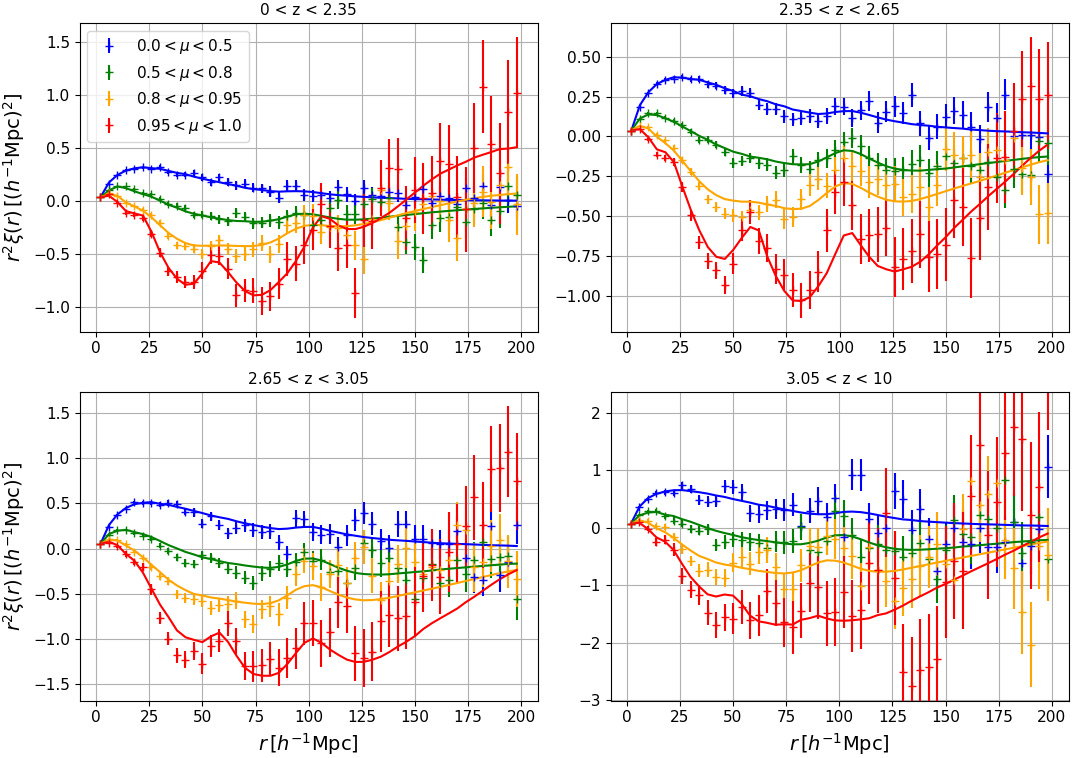
\includegraphics[scale=0.4]{dr16_4bins}
  \caption{Fonctions de corrélation \lya{}$\times$\lya{} dans chacun des bins en redshift de l'analyse. Les courbes en trait plein donne le meilleur ajustement du modèle obtenu avec \texttt{picca}. Chaque graphique correspond à un bin en redshift. Pour chacun des bins, la fonction de corrélation et l'ajustement sont montrés dans quatre bins en $\mu$.}
  \label{fig:dr16_4bins}
\end{figure}

\begin{table}[]
  \centering
  \caption{Résultats de l'ajustement fait avec \texttt{picca} des fonctions de corrélation \lya{}$\times$\lya{} calculées sur les données DR16. Chaque colonne donne le résultat de l'ajustement d'un bin en redshift. La dernière colonne donne le résultat de l'ajustement de la corrélation moyennée sur ces quatre bins en redshift. La première section du tableau donne les paramètres du modèle qui sont ajustés. La seconde donne le $\chi^2$ et le redshift effectif $z_{\mathrm{eff}}$. Le modèle comporte \num{13} paramètres libres. Le nombre de bins sur lesquels le modèle est ajusté est $N_{bin} = \num{1590}$, ce qui donne un nombre de degrés de liberté $n_{d.o.f.} = \num{1577}$. Enfin, la dernière section donne le biais et le biais effectif du \lya{}. Ils sont reliés aux paramètres $b_{\eta, \mathrm{Ly}\alpha}$ et $\beta_{\mathrm{Ly}\alpha}$ par les équations~\ref{eq:def_bias} et~\ref{eq:def_bias_eff}.}
  \label{tab:dr16_4bins}
  \footnotesize
  \begin{tabular}{lccccc}
    % \toprule
    % Paramètre  & $\num{0} < z < \num{2.35}$ & $\num{2.35} < z < \num{2.65}$ & $\num{2.65} < z < \num{3.05}$ & $\num{3.05} < z < \num{10}$ \\
    % \midrule
    % $\apar{}$ & 1.0626413422656635 +/- 0.06560781661781079 & 1.0188646800560925 +/- 0.041362422911403685 & 1.029148212201299 +/- 0.07242396192712802 & 1.1200171298229007 +/- 0.08091370899309824 \\
    % $\aper{}$ & 1.0632375535901253 +/- 0.10810794059323114 & 0.9652958910718991 +/- 0.057180394974236104 & 1.0159330757036005 +/- 0.05784775528375763 0.9255146850435335 +/- 0.07206257341759192 \\
    % $b_{\eta, \mathrm{Ly}\alpha}$ & -0.1795977211203897 +/- 0.005769053847991895 & -0.19377778657236358 +/- 0.00526939132784233 & -0.2236876829818197 +/- 0.008421287322167362 & -0.2928514012382003 +/- 0.018740373333761263 \\
    % $\beta_{\mathrm{Ly}\alpha}$ & 2.093809306317262 +/- 0.210449292900992 & 1.7112686242434043 +/- 0.13322965498374356 & 1.4274033068601393 +/- 0.13841133835520955 & 1.264422978848562 +/- 0.19412583530626168 \\
    % $10^3 b_{\eta, \mathrm{SiII}(1190)}$ & -0.0018292445000232958 +/- 0.0010951582472295686 & -0.003656308599416015 +/- 0.0006752880865250276 & -0.002801629741142273 +/- 0.0010118710088140865 & 0.00036032759305010395 +/- 0.0016376260200395207 \\
    % $10^3 b_{\eta, \mathrm{SiII}(1193)}$ & -0.004830928957010919 +/- 0.001100315153087375 & -0.0019362727878605114 +/- 0.0006919289269201215 & -0.0007847568940101366 +/- 0.0009691126424570403 & -0.002131181997407055 +/- 0.0017224737321217046 \\
    % $10^3 b_{\eta, \mathrm{SiII}(1260)}$ & -0.003375467125024695 +/- 0.0013329581881429706 &  -0.001969961682619123 +/- 0.000795815740207674 & -0.001317200522029868 +/- 0.0010526150274975418 & 0.0008965020540008499 +/- 0.001791480805493678 \\
    % $10^3 b_{\eta, \mathrm{SiIII}(1207)}$ &  -0.007865921480598285 +/- 0.0011034826815558326 & -0.004523595559873886 +/- 0.0007456098975624773 & -0.0021082960921853036 +/- 0.001047671905738136 & -0.0028969289782045586 +/- 0.001740041127658313 \\
    % $10^3 b_{\eta, CIV(eff)}$ & -0.004767305959965107 +/- 0.002544174250674547 & -0.005150878411363191 +/- 0.002643560029682246 & -0.005060576315171872 +/- 0.0026177990462492584 & -0.005022340903756195 +/- 0.002605282928692776 \\
    % $b_{\textsc{HCD}}$ & -0.05959772317290102 +/- 0.007001888877137152 & -0.04517388629736585 +/- 0.0060459072913988665 & -0.06651201389736294 +/- 0.010015445096663855 & -0.022781727665758256 +/- 0.021820968368492788 \\
    % $\beta_{\textsc{HCD}}$ & 0.5513755924633041 +/- 0.08641628187515504 & 0.55971852703097 +/- 0.08649826856663473 & 1.4274033068601393 +/- 0.13841133835520955 & 0.5026113732660472 +/- 0.08990286553465421 \\
    % $10^2 A_{sky}$ & 0.015852430760394755 +/- 0.0009832458229809115 & 0.008702223782589641 +/- 0.000816825935201006 & 0.007285381419552714 +/- 0.0013334299368094303 & 0.006448552548337415 +/- 0.0033839253887543966 \\
    % $\sigma_{sky}$ & 32.542936141293126 +/- 1.7910999585024947 & 31.590693919063543 +/- 2.5612829757179214 & 31.930967631996463 +/- 4.270238324140993
    % \bottomrule & 34.1693831220765 +/- 16.09450395736028 \\

    % $\apar{}$ & 1.0626413422656635 +/- 0.06560781661781079 & 1.0188646800560925 +/- 0.041362422911403685 & 1.029148212201299 +/- 0.07242396192712802 & 1.1200171298229007 +/- 0.08091370899309824 \\
    % $\aper{}$ & 1.0632375535901253 +/- 0.10810794059323114 & 0.9652958910718991 +/- 0.057180394974236104 & 1.0159330757036005 +/- 0.05784775528375763 0.9255146850435335 +/- 0.07206257341759192 \\
    % $b_{\eta, \mathrm{Ly}\alpha}$ & -0.1795977211203897 +/- 0.005769053847991895 & -0.19377778657236358 +/- 0.00526939132784233 & -0.2236876829818197 +/- 0.008421287322167362 & -0.2928514012382003 +/- 0.018740373333761263 \\
    % $\beta_{\mathrm{Ly}\alpha}$ & 2.093809306317262 +/- 0.210449292900992 & 1.7112686242434043 +/- 0.13322965498374356 & 1.4274033068601393 +/- 0.13841133835520955 & 1.264422978848562 +/- 0.19412583530626168 \\
    % $10^3 b_{\eta, \mathrm{SiII}(1190)}$ & -1.8292445000232958 +/- 1.0951582472295686 & -3.656308599416015 +/- 0.6752880865250276 & -2.801629741142273 +/- 1.0118710088140865 & 0.36032759305010395 +/- 1.6376260200395207 \\
    % $10^3 b_{\eta, \mathrm{SiII}(1193)}$ & -4.830928957010919 +/- 1.100315153087375 & -1.9362727878605114 +/- 0.6919289269201215 & -0.7847568940101366 +/- 0.9691126424570403 & -2.131181997407055 +/- 1.7224737321217046 \\
    % $10^3 b_{\eta, \mathrm{SiII}(1260)}$ & -3.375467125024695 +/- 1.3329581881429706 &  -1.969961682619123 +/- 0.795815740207674 & -1.317200522029868 +/- 1.0526150274975418 & 0.8965020540008499 +/- 1.791480805493678 \\
    % $10^3 b_{\eta, \mathrm{SiIII}(1207)}$ &  -7.865921480598285 +/- 1.1034826815558326 & -4.523595559873886 +/- 0.7456098975624773 & -2.1082960921853036 +/- 1.047671905738136 & -2.8969289782045586 +/- 1.740041127658313 \\
    % $10^3 b_{\eta, CIV(eff)}$ & -4.767305959965107 +/- 2.544174250674547 & -5.150878411363191 +/- 2.643560029682246 & -5.060576315171872 +/- 2.6177990462492584 & -5.022340903756195 +/- 2.605282928692776 \\
    % $b_{\textsc{HCD}}$ & -0.05959772317290102 +/- 0.007001888877137152 & -0.04517388629736585 +/- 0.0060459072913988665 & -0.06651201389736294 +/- 0.010015445096663855 & -0.022781727665758256 +/- 0.021820968368492788 \\
    % $\beta_{\textsc{HCD}}$ & 0.5513755924633041 +/- 0.08641628187515504 & 0.55971852703097 +/- 0.08649826856663473 & 1.4274033068601393 +/- 0.13841133835520955 & 0.5026113732660472 +/- 0.08990286553465421 \\
    % $10^2 A_{sky}$ & 1.5852430760394755 +/- 0.09832458229809115 & 0.8702223782589641 +/- 0.0816825935201006 & 0.7285381419552714 +/- 0.13334299368094303 & 0.6448552548337415 +/- 0.33839253887543966 \\
    % $\sigma_{sky}$ & 32.542936141293126 +/- 1.7910999585024947 & 31.590693919063543 +/- 2.5612829757179214 & 31.930967631996463 +/- 4.270238324140993
    % \bottomrule & 34.1693831220765 +/- 16.09450395736028 \\

%     $\apar{} $ & $ 1.063 \pm 0.066 $ & $ 1.019 \pm 0.041 $ & $ 1.029 \pm 0.072 $ & $ 1.120 \pm 0.081 $ \\
%     $\aperp{} $ & $ 1.063 \pm 0.108 $ & $ 0.965 \pm 0.057 $ & $ 1.016 \pm 0.058 $ & $ 0.926 \pm 0.072 $ \\
%     $b_{\eta, \mathrm{Ly}\alpha} $ & $ -0.1796 \pm 0.0058 $ & $ -0.1938 \pm 0.0053 $ & $ -0.2239 \pm 0.0084 $ & $ -0.2929 \pm 0.0187 $ \\
%     $\beta_{\mathrm{Ly}\alpha} $ & $ 2.094 \pm 0.210 $ & $ 1.711 \pm 0.133 $ & $ 1.427 \pm 0.138 $ & $ 1.264 \pm 0.194 $ \\
%     $10^3 b_{\eta, \mathrm{SiII}(1190)} $ & $ -1.83 \pm 1.10 $ & $ -3.66 \pm 0.68 $ & $ -2.80 \pm 1.01 $ & $ 0.36 \pm 1.64 $ \\
%     $10^3 b_{\eta, \mathrm{SiII}(1193)} $ & $ -4.83 \pm 1.10 $ & $ -1.94 \pm 0.69 $ & $ -0.78 \pm 0.97 $ & $ -2.13 \pm 1.72 $\\
%     $10^3 b_{\eta, \mathrm{SiII}(1260)} $ & $ -3.38 \pm 1.33 $ & $  -1.97 \pm 0.80 $ & $ -1.32 \pm 1.05 $ & $ 0.90 \pm 1.79 $\\
%     $10^3 b_{\eta, \mathrm{SiIII}(1207)} $ & $  -7.87 \pm 1.10 $ & $ -4.52 \pm 0.74 $ & $ -2.11 \pm 1.05 $ & $ -2.90 \pm 1.74 $\\
%     $10^3 b_{\eta, CIV(\mathrm{eff})} $ & $ -4.77 \pm 2.54 $ & $ -5.15 \pm 2.64 $ & $ -5.06 \pm 2.62 $ & $ -5.02 \pm 2.61 $\\
%     $b_{\textsc{HCD}} $ & $ -0.0596 \pm 0.0070 $ & $ -0.0452 \pm 0.0060 $ & $ -0.0665 \pm 0.0100 $ & $ -0.0228 \pm 0.0218 $\\
%     $\beta_{\textsc{HCD}} $ & $ 0.551 \pm 0.086 $ & $ 0.560 \pm 0.086 $ & $ 0.508 \pm 0.088 $ & $ 0.503 \pm 0.090 $\\
%     $10^2 A_{sky} $ & $ 1.585 \pm 0.098 $ & $ 0.870 \pm 0.082 $ & $ 0.729 \pm 0.133 $ & $ 0.645 \pm 0.338 $\\
%     $\sigma_{sky} $ & $ 32.5 \pm 1.7 $ & $ 31.6 \pm 2.6 $ & $ 31.9 \pm 4.3 $ & $ 34.2 \pm 16.1 $\\
%     \midrule
%     $\chi^2$ & 1568.33 & 1512.33 & 1680.82 & 1674.59 \\
%     \midrule
%     $b_{\mathrm{Ly}\alpha} $ & $ -0.0832 \pm -0.0065 $ & $ -0.1099 \pm -0.0063 $ & $ -0.1521 \pm -0.01025 $ & $ -0.2248 \pm -0.0230 $\\
%     $b_{\mathrm{eff}, \mathrm{Ly}\alpha} $ & $ -0.1506 \pm 0.0046 $ & $ -0.1814 \pm 0.0045 $ & $ -0.2336 \pm 0.0074 $ & $ -0.3305 \pm 0.0169 $\\
%     \bottomrule
% \toprule
% Param\`etre  & $\num{0} < z < \num{2.35}$ & $\num{2.35} < z < \num{2.65}$ & $\num{2.65} < z < \num{3.05}$ & $\num{3.05} < z < \num{10}$ \\
% \midrule
% $\apar{} $ & $ 1.063 \pm 0.066$ & $ 1.019 \pm 0.041$ & $ 1.029 \pm 0.072$ & $ 1.12 \pm 0.081$ \\
% $\aperp{} $ & $ 1.063 \pm 0.108$ & $ 0.965 \pm 0.057$ & $ 1.016 \pm 0.058$ & $ 0.926 \pm 0.072$ \\
% $b_{\eta, \mathrm{Ly}\alpha} $ & $ -0.1796 \pm 0.0058$ & $ -0.1938 \pm 0.0053$ & $ -0.2237 \pm 0.0084$ & $ -0.2929 \pm 0.0187$ \\
% $\beta_{\mathrm{Ly}\alpha} $ & $ 2.094 \pm 0.21$ & $ 1.711 \pm 0.133$ & $ 1.427 \pm 0.138$ & $ 1.265 \pm 0.194$ \\
% $10^3 b_{\eta, \mathrm{SiII}(1190)} $ & $ -1.83 \pm 1.1$ & $ -3.66 \pm 0.68$ & $ -2.8 \pm 1.01$ & $ 0.36 \pm 1.64$ \\
% $10^3 b_{\eta, \mathrm{SiII}(1193)} $ & $ -4.83 \pm 1.1$ & $ -1.94 \pm 0.69$ & $ -0.79 \pm 0.97$ & $ -2.13 \pm 1.72$ \\
% $10^3 b_{\eta, \mathrm{SiII}(1260)} $ & $ -3.38 \pm 1.33$ & $ -1.97 \pm 0.8$ & $ -1.32 \pm 1.05$ & $ 0.9 \pm 1.79$ \\
% $10^3 b_{\eta, \mathrm{SiIII}(1207)} $ & $ -7.87 \pm 1.1$ & $ -4.52 \pm 0.75$ & $ -2.11 \pm 1.05$ & $ -2.89 \pm 1.74$ \\
% $10^3 b_{\eta, CIV(\mathrm{eff})} $ & $ -4.77 \pm 2.54$ & $ -5.15 \pm 2.64$ & $ -5.06 \pm 2.62$ & $ -5.02 \pm 2.61$ \\
% $b_{\textsc{HCD}} $ & $ -0.0596 \pm 0.007$ & $ -0.0452 \pm 0.006$ & $ -0.0665 \pm 0.01$ & $ -0.0228 \pm 0.0218$ \\
% $\beta_{\textsc{HCD}} $ & $ 0.551 \pm 0.086$ & $ 0.56 \pm 0.086$ & $ 0.508 \pm 0.088$ & $ 0.502 \pm 0.09$ \\
% $10^2 A_{sky} $ & $ 1.585 \pm 0.098$ & $ 0.87 \pm 0.082$ & $ 0.729 \pm 0.133$ & $ 0.646 \pm 0.338$ \\
% $\sigma_{sky} $ & $ 32.5 \pm 1.8$ & $ 31.6 \pm 2.6$ & $ 31.9 \pm 4.3$ & $ 34.1 \pm 16.0$ \\
% \midrule
% $\chi^2$ & $ 1568 $ & $ 1512 $ & $ 1681 $ & $ 1675 $ \\
% $z_{\mathrm{eff}}$ & $ 2.136 $ & $ 2.276 $ & $ 2.551 $ & $ 2.914 $ \\
% \midrule
% $b_{\mathrm{Ly}\alpha} $ & $ -0.0832 \pm 0.0065$ & $ -0.1099 \pm 0.0063$ & $ -0.1521 \pm 0.0103$ & $ -0.2247 \pm 0.023$ \\
% $b_{\mathrm{eff}, \mathrm{Ly}\alpha} $ & $ -0.1506 \pm 0.0046$ & $ -0.1814 \pm 0.0045$ & $ -0.2336 \pm 0.0074$ & $ -0.3305 \pm 0.0168$ \\
% \bottomrule
% \toprule
% Param\`etre  & $\num{0} < z < \num{2.35}$ & $\num{2.35} < z < \num{2.65}$ & $\num{2.65} < z < \num{3.05}$ & $\num{3.05} < z < \num{10}$ \\
% \midrule
% $\apar{} $ & $ 1.063 \pm 0.066$ & $ 1.019 \pm 0.041$ & $ 1.029 \pm 0.072$ & $ 1.12 \pm 0.081$ \\
% $\aperp{} $ & $ 1.063 \pm 0.108$ & $ 0.965 \pm 0.057$ & $ 1.016 \pm 0.058$ & $ 0.926 \pm 0.072$ \\
% $b_{\eta, \mathrm{Ly}\alpha} $ & $ -0.1796 \pm 0.0058$ & $ -0.1938 \pm 0.0053$ & $ -0.2237 \pm 0.0084$ & $ -0.2929 \pm 0.0187$ \\
% $\beta_{\mathrm{Ly}\alpha} $ & $ 2.094 \pm 0.21$ & $ 1.711 \pm 0.133$ & $ 1.427 \pm 0.138$ & $ 1.265 \pm 0.194$ \\
% $10^3 b_{\eta, \mathrm{SiII}(1190)} $ & $ -1.83 \pm 1.1$ & $ -3.66 \pm 0.68$ & $ -2.8 \pm 1.01$ & $ 0.36 \pm 1.64$ \\
% $10^3 b_{\eta, \mathrm{SiII}(1193)} $ & $ -4.83 \pm 1.1$ & $ -1.94 \pm 0.69$ & $ -0.79 \pm 0.97$ & $ -2.13 \pm 1.72$ \\
% $10^3 b_{\eta, \mathrm{SiII}(1260)} $ & $ -3.38 \pm 1.33$ & $ -1.97 \pm 0.8$ & $ -1.32 \pm 1.05$ & $ 0.9 \pm 1.79$ \\
% $10^3 b_{\eta, \mathrm{SiIII}(1207)} $ & $ -7.87 \pm 1.1$ & $ -4.52 \pm 0.75$ & $ -2.11 \pm 1.05$ & $ -2.89 \pm 1.74$ \\
% $10^3 b_{\eta, CIV(\mathrm{eff})} $ & $ -4.77 \pm 2.54$ & $ -5.15 \pm 2.64$ & $ -5.06 \pm 2.62$ & $ -5.02 \pm 2.61$ \\
% $b_{\textsc{HCD}} $ & $ -0.0596 \pm 0.007$ & $ -0.0452 \pm 0.006$ & $ -0.0665 \pm 0.01$ & $ -0.0228 \pm 0.0218$ \\
% $\beta_{\textsc{HCD}} $ & $ 0.551 \pm 0.086$ & $ 0.56 \pm 0.086$ & $ 0.508 \pm 0.088$ & $ 0.502 \pm 0.09$ \\
% $10^2 A_{sky} $ & $ 1.585 \pm 0.098$ & $ 0.87 \pm 0.082$ & $ 0.729 \pm 0.133$ & $ 0.646 \pm 0.338$ \\
% $\sigma_{sky} $ & $ 32.5 \pm 1.8$ & $ 31.6 \pm 2.6$ & $ 31.9 \pm 4.3$ & $ 34.1 \pm 16.0$ \\
% \midrule
% $\chi^2$ & $ 1568 $ & $ 1512 $ & $ 1681 $ & $ 1675 $ \\
% $z_{\mathrm{eff}}$ & $ 2.136 $ & $ 2.276 $ & $ 2.551 $ & $ 2.914 $ \\
% \midrule
% $b_{\mathrm{Ly}\alpha} $ & $ -0.0832 \pm 0.0065$ & $ -0.1099 \pm 0.0063$ & $ -0.1521 \pm 0.0103$ & $ -0.2247 \pm 0.023$ \\
% $b_{\mathrm{eff}, \mathrm{Ly}\alpha} $ & $ -0.1506 \pm 0.0046$ & $ -0.1814 \pm 0.0045$ & $ -0.2336 \pm 0.0074$ & $ -0.3305 \pm 0.0168$ \\
% \bottomrule
\toprule
Param\`etre  & $\num{0} < z < \num{2.35}$ & $\num{2.35} < z < \num{2.65}$ & $\num{2.65} < z < \num{3.05}$ & $\num{3.05} < z < \num{10}$  & $\num{0} < z < \num{10}$ \\
\midrule
$\apar{} $ & $ 1.063 \pm 0.066$ & $ 1.019 \pm 0.041$ & $ 1.029 \pm 0.072$ & $ 1.120 \pm 0.081$ & $ 1.047 \pm 0.034$ \\
$\aperp{} $ & $ 1.063 \pm 0.108$ & $ 0.965 \pm 0.057$ & $ 1.016 \pm 0.058$ & $ 0.926 \pm 0.072$ & $ 0.980 \pm 0.042$ \\
$b_{\eta, \mathrm{Ly}\alpha} $ & $ -0.1796 \pm 0.0058$ & $ -0.1938 \pm 0.0053$ & $ -0.2237 \pm 0.0084$ & $ -0.2929 \pm 0.0187$ & $ -0.1998 \pm 0.0039$ \\
$\beta_{\mathrm{Ly}\alpha} $ & $ 2.094 \pm 0.210$ & $ 1.711 \pm 0.133$ & $ 1.427 \pm 0.138$ & $ 1.265 \pm 0.194$ & $ 1.633 \pm 0.087$ \\
$10^3 b_{\eta, \mathrm{SiII}(1190)} $ & $ -1.83 \pm 1.10$ & $ -3.66 \pm 0.68$ & $ -2.80 \pm 1.01$ & $ 0.36 \pm 1.64$ & $ -3.02 \pm 0.51$ \\
$10^3 b_{\eta, \mathrm{SiII}(1193)} $ & $ -4.83 \pm 1.10$ & $ -1.94 \pm 0.69$ & $ -0.79 \pm 0.97$ & $ -2.13 \pm 1.72$ & $ -2.07 \pm 0.50$ \\
$10^3 b_{\eta, \mathrm{SiII}(1260)} $ & $ -3.38 \pm 1.33$ & $ -1.97 \pm 0.80$ & $ -1.32 \pm 1.05$ & $ 0.90 \pm 1.79$ & $ -2.16 \pm 0.63$ \\
$10^3 b_{\eta, \mathrm{SiIII}(1207)} $ & $ -7.87 \pm 1.10$ & $ -4.52 \pm 0.75$ & $ -2.11 \pm 1.05$ & $ -2.89 \pm 1.74$ & $ -4.59 \pm 0.52$ \\
$10^3 b_{\eta, CIV(\mathrm{eff})} $ & $ -4.77 \pm 2.54$ & $ -5.15 \pm 2.64$ & $ -5.06 \pm 2.62$ & $ -5.02 \pm 2.61$ & $ -5.12 \pm 2.63$ \\
$b_{\textsc{HCD}} $ & $ -0.0596 \pm 0.0070$ & $ -0.0452 \pm 0.0060$ & $ -0.0665 \pm 0.0100$ & $ -0.0228 \pm 0.0218$ & $ -0.0521 \pm 0.0045$ \\
$\beta_{\textsc{HCD}} $ & $ 0.551 \pm 0.086$ & $ 0.560 \pm 0.086$ & $ 0.508 \pm 0.088$ & $ 0.502 \pm 0.090$ & $ 0.603 \pm 0.083$ \\
$10^2 A_{sky} $ & $ 1.585 \pm 0.098$ & $ 0.870 \pm 0.082$ & $ 0.729 \pm 0.133$ & $ 0.646 \pm 0.338$ & $ 0.947 \pm 0.060$ \\
$\sigma_{sky} $ & $ 32.5 \pm 1.8$ & $ 31.6 \pm 2.6$ & $ 31.9 \pm 4.3$ & $ 34.1 \pm 16.0$ & $ 31.4 \pm 1.7$ \\
\midrule
$\chi^2$ & $ 1568 $ & $ 1512 $ & $ 1681 $ & $ 1675 $ & $ 1602 $ \\
$z_{\mathrm{eff}}$ & $ 2.136 $ & $ 2.276 $ & $ 2.551 $ & $ 2.914 $ & $ 2.334 $ \\
\midrule
$b_{\mathrm{Ly}\alpha} $ & $ -0.0832 \pm 0.0065$ & $ -0.1099 \pm 0.0063$ & $ -0.1521 \pm 0.0103$ & $ -0.2247 \pm 0.0230$ & $ -0.1187 \pm 0.0046$ \\
$b_{\mathrm{eff}, \mathrm{Ly}\alpha} $ & $ -0.1506 \pm 0.0046$ & $ -0.1814 \pm 0.0045$ & $ -0.2336 \pm 0.0074$ & $ -0.3305 \pm 0.0168$ & $ -0.1922 \pm 0.0033$ \\
\bottomrule
\end{tabular}
\end{table}


La figure~\ref{fig:dr16_4bins} présente la fonction de corrélation et le meilleur ajustement du modèle dans chacun des bins en redshift. Les différents graphiques montrent les différents bins en redshift. Dans chaque graphique, la fonction de corrélation est affichée dans quatre bins en $\mu$. Le tableau~\ref{tab:dr16_4bins} donne le résultat de l'ajustement dans chacun des bins en redshift, ainsi que l'ajustement fait sur la corrélation moyennée sur ces bins.
% La première section du tableau donne les paramètres ajustés, la deuxième donne le redshift effectif $z_{\mathrm{eff}}$ et le $\chi^2$ obtenu. Le nombre de bins dans lesquels la fonction de corrélation est ajustée est $N_{bin} = \num{1590}$, ce qui donne un nombre de degrés de liberté $N_{d.o.f.} = \num{1590} - \num{13} = \num{1577}$. Enfin, la troisième colonne donne le biais et le biais effectif du \lya{}.
% Le biais $b_{\mathrm{Ly}\alpha} $ est obtenu comme
% \begin{equation}
%   \label{eq:def_bias}
%   b_{\mathrm{Ly}\alpha}  = \frac{b_{\eta, \mathrm{Ly}\alpha} f}{\beta_{\mathrm{Ly}\alpha}} \; .
% \end{equation}
% Le biais effectif $b_{\mathrm{eff}, \mathrm{Ly}\alpha} $ est défini comme
% \begin{equation}
%   \label{eq:def_bias_eff}
%   b_{\mathrm{eff}, \mathrm{Ly}\alpha} = b_{\mathrm{Ly}\alpha} \sqrt{1 + \frac{2}{3} \beta_{\mathrm{Ly}\alpha} + \frac{1}{5} \beta_{\mathrm{Ly}\alpha}^2} \; .
% \end{equation}
% Il est sensible à l'amplitude de la fonction de corrélation, et est moins corrélé avec $\beta_{\mathrm{Ly}\alpha}$ que l'est $b_{\eta, \mathrm{Ly}\alpha}$ ou $b_{\mathrm{Ly}\alpha}$ (\#prov doublon avec le chap4).
Une fois cette analyse produite, et toujours dans le but d'obtenir $b_{\mathrm{eff},\mathrm{Ly}\alpha}(z)$ et $\beta_{\mathrm{Ly}\alpha}(z)$ pour $\num{1.9} < z  < \num{3.6}$, nous ajustons les paramètres \lya{} mesurés dans les données par une loi de puissance. La figure~\ref{fig:bias_vs_z} présente les mesures $b_{\mathrm{eff},\mathrm{Ly}\alpha}$ et $\beta_{\mathrm{Ly}\alpha}$ dans les quatre bins en redshift, ainsi que l'ajustement fait sur ces quatres points.
% Pour le biais effectif, nous obtenons $b_{\mathrm{eff},\mathrm{Ly}\alpha}(z) \propto (1+z)^{\gamma}$ avec $\gamma = \num{3.474} \pm \num{0.025}$.
Pour le biais effectif, nous obtenons $b_{\mathrm{eff},\mathrm{Ly}\alpha}(z) = A (1+z)^{\gamma}$ avec $A = \num{0.0029} \pm \num{0.0009}$ et $\gamma = \num{3.47} \pm \num{0.26}$.
% Pour le paramètre RSD, nous obtenons $\beta_{\mathrm{Ly}\alpha}(z) \propto (1+z)^{\gamma}$ avec $\gamma = - \num{2.32} \pm \num{1.97}$.
Pour le paramètre RSD, nous obtenons $\beta_{\mathrm{Ly}\alpha}(z) = A (1+z)^{\gamma}$ avec $A = \num{27.7} \pm \num{47.1}$ et $\gamma = - \num{2.32} \pm \num{1.40}$.
Ces deux ajustements sont utilisés comme référence pour l'ajustement des paramètres des mocks (section~\ref{sec:tuning}). Ils sont extrapolés de $z = \num{1.9}$ jusqu'à $z = \num{3.6}$.


\begin{figure}
  \centering
  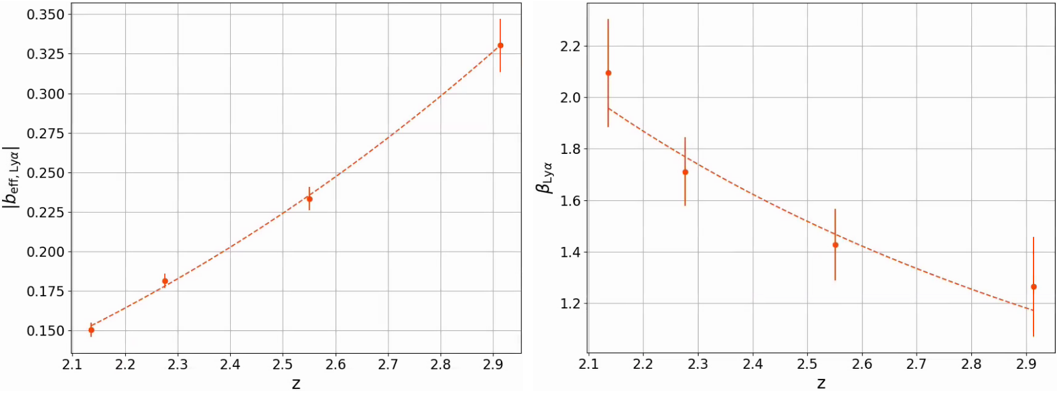
\includegraphics[scale=0.44]{bias_vs_z}
  \caption{Mesure des paramètres $b_{\mathrm{eff},\mathrm{Ly}\alpha}$ et $\beta_{\mathrm{Ly}\alpha}$ dans les données DR16. Les mesures sont faites dans quatre bins en redshift, indiquées par les points. La ligne en pointillés donne le meilleur ajustement par une loi de puissance.}
  % Cet ajustement donne $b_{\mathrm{eff},\mathrm{Ly}\alpha}(z) \propto (1+z)^{\gamma}$ avec $\gamma = \num{3.474} \pm \num{0.025}$ et $\beta_{\mathrm{Ly}\alpha}(z) \propto (1+z)^{\gamma}$ avec $\gamma = - \num{2.32} \pm \num{1.97}$.}
  \label{fig:bias_vs_z}
\end{figure}





\subsection{Stabilité des paramètres \lya{}}
\label{subsec:stab_pars_lya}


\begin{table}[]
  \centering
  \caption{Corrélations des paramètres du modèle avec les paramètres $b_{\eta,\mathrm{Ly}\alpha}$ et $\beta_{\mathrm{Ly}\alpha}$ lors de l'ajustement de la fonction de corrélation \lya{}$\times$\lya{}. L'ajustement est fait sur la moyenne des fonctions de corrélation calculées dans chaque bin en redshift, soit l'ensemble des données DR16.}
  \label{tab:corr_bias_lya}
  \begin{tabular}{lcc}
    \toprule
    Paramètre  & $b_{\eta,\mathrm{Ly}\alpha}$ & $\beta_{\mathrm{Ly}\alpha}$ \\
    \midrule
    $\apar{} $ & \SI{-0}{\percent} & \SI{0}{\percent}\\
    $\aperp{} $ & \SI{1}{\percent} & \SI{-2}{\percent} \\
    $b_{\eta, \mathrm{Ly}\alpha} $ & \SI{100}{\percent} & \SI{-87}{\percent} \\
    $\beta_{\mathrm{Ly}\alpha} $ & \SI{-87}{\percent} &  \SI{100}{\percent} \\
    $b_{\eta, \mathrm{SiII}(1190)} $ & \SI{2}{\percent} & \SI{-8}{\percent} \\
    $b_{\eta, \mathrm{SiII}(1193)} $ & \SI{3}{\percent} & \SI{-6}{\percent} \\
    $b_{\eta, \mathrm{SiII}(1260)} $ & \SI{-1}{\percent} & \SI{-3}{\percent} \\
    $b_{\eta, \mathrm{SiIII}(1207)} $ & \SI{6}{\percent} & \SI{5}{\percent}\\
    $b_{\eta, CIV(\mathrm{eff})} $ &\SI{-7}{\percent} & \SI{-10}{\percent}\\
    $b_{\textsc{HCD}} $ & \SI{48}{\percent} & \SI{-75}{\percent}\\
    $\beta_{\textsc{HCD}} $ & \SI{35}{\percent} & \SI{-23}{\percent}\\
    $A_{sky} $ & \SI{34}{\percent} & \SI{-19}{\percent}\\
    $\sigma_{sky} $ & \SI{-10}{\percent} & \SI{-2}{\percent}\\
    \bottomrule
\end{tabular}
\end{table}

% \begin{table}[]
%   \centering
%   \caption{Corrélations des paramètres du modèle avec le paramètre $\beta_{\mathrm{Ly}\alpha}$ lors de l'ajustement de la fonction de corrélation \lya{}$\times$\lya{}. L'ajustement est fait sur l'addition des fonctions de corrélation calculées dans chaque bin en redshift, soit l'ensemble des données DR16.}
%   \label{tab:corr_beta_lya}
%   \begin{tabular}{lr}
%     \toprule
%     Paramètre  & Corrélation avec $\beta_{\mathrm{Ly}\alpha}$ \\
%     \midrule
%     $\apar{} $ & \SI{0}{\percent}\\
%     $\aperp{} $ & \SI{-2}{\percent} \\
%     $b_{\eta, \mathrm{Ly}\alpha} $ & \SI{-87}{\percent} \\
%     $\beta_{\mathrm{Ly}\alpha} $ & \SI{100}{\percent} \\
%     $10^3 b_{\eta, \mathrm{SiII}(1190)} $ & \SI{-8}{\percent} \\
%     $10^3 b_{\eta, \mathrm{SiII}(1193)} $ & \SI{-6}{\percent} \\
%     $10^3 b_{\eta, \mathrm{SiII}(1260)} $ & \SI{-3}{\percent} \\
%     $10^3 b_{\eta, \mathrm{SiIII}(1207)} $ & \SI{5}{\percent} \\
%     $10^3 b_{\eta, CIV(\mathrm{eff})} $ &\SI{-10}{\percent} \\
%     $b_{\textsc{HCD}} $ & \SI{-75}{\percent} \\
%     $\beta_{\textsc{HCD}} $ & \SI{-23}{\percent} \\
%     $10^2 A_{sky} $ & \SI{-19}{\percent} \\
%     $\sigma_{sky} $ & \SI{-2}{\percent} \\
%     \bottomrule
% \end{tabular}
% \end{table}
Après avoir produit les ajustements présentés dans la section précédente, nous avons cherché à savoir si la mesure des paramètres \lya{} était fiable. Nous avons d'abord regardé la corrélation des paramètres $b_{\eta,\mathrm{Ly}\alpha}$ et $\beta_{\mathrm{Ly}\alpha}$ avec les autres paramètres du modèle. La table~\ref{tab:corr_bias_lya} présente ces corrélations.
Premièrement, nous pouvons remarquer que les deux paramètres \lya{} ajustés sont très anticorrélés : \SI{-87}{\percent}.
% Il serait intéressant d'étudier quel couple de paramètres sont les moins corrélés.
% Ceci vient du fait que le paramètre RSD du \lya{} est très important : le signal se trouve principalement le long de la ligne de visée. Avec peu de signal perpendiculairement à la ligne de visée, il est difficile de décorréler le biais du paramètre RSD du traceur.
Deuxièmement, les paramètres du \lya{} sont très corrélés avec ceux des HCD, notament $\beta_{\mathrm{Ly}\alpha}$ qui est corrélé à \SI{-75}{\percent} avec $b_{\textsc{HCD}}$.
% Ceci pose plusieurs problèmes : d'abord, la modélisation des HCD choisie dans \textcite{DuMasdesBourboux2020} et utilisée ici consiste à identifier puis masquer les HCD avec $\log n_{\textsc{HI}} > \num{20.3}$, les HCD non masqués étant pris en compte par le terme $F_{\textsc{HCD}}$ (voir section~\ref{subsec:model_donnees}).
Ceci pose plusieurs problèmes : d'abord, la modélisation des HCD choisie dans \textcite{DuMasdesBourboux2020} et utilisée ici consiste à masquer les HCD identifiés par un algorithme. En pratique cela revient à masquer les HCD avec une densité de colonne $\log n_{\textsc{HI}} > \num{20.3}$. Les HCD non masqués sont pris en compte par le terme $F_{\textsc{HCD}}$ (voir section~\ref{subsec:model_donnees}).
Cependant, l'algorithme utilisé ne possède pas une efficacité de \SI{100}{\percent} (Chabanier et al. (in prep)). Des HCD avec une grande densité de colonne ne sont donc pas masqués.
Ces HCD produisent des absorptions intenses, non prises en compte par le terme $F_{\textsc{HCD}}$, ce qui a pour effet d'augmenter le biais du \lya{}.
% Ensuite, le paramètre effectif $L_{\textsc{HCD}}$ est fixé à \SI{10}{\perh\Mpc} car il est corrélé avec les autres paramètres.
Ensuite, le paramètre effectif $L_{\textsc{HCD}}$ doit être fixé car il est très corrélé avec les autres paramètres (voir le paragraphe suivant).
Sa valeur, qui dépend de la distribution des HCD non masqués, est difficile à déterminer.
Une valeur de \SI{10}{\perh\Mpc} a été choisie dans l’analyse DR16, de façon un peu arbitraire dans la mesure où cela n’affecte pas la mesure de l’échelle BAO.
% Du fait des corrélations avec les autres paramètres, le fait de changer $L_{\textsc{HCD}}$ change la valeur de $b_{\textsc{HCD}}$.
% Du fait des corrélations avec les autres paramètres, les paramètres des HCD obtenus dépendent de la valeur de $L_{\textsc{HCD}}$ choisie.
% La figure~\ref{fig:bias_hcd_vs_L0_dr16} montre la dépendance de $b_{\textsc{HCD}}$ et $\beta_{\textsc{HCD}}$ avec $L_{\textsc{HCD}}$.

Nous remarquons que les paramètres des HCD obtenus dépendent de la valeur de $L_{\textsc{HCD}}$ choisie, comme illustré sur la figure~\ref{fig:bias_hcd_vs_L0_dr16}.
A cause des corrélations entre les paramètres liés aux HCD et ceux liés au \lya{}, le fait de changer $L_{\textsc{HCD}}$ change aussi les paramètres \lya{} obtenus.
La figure~\ref{fig:bias_lya_vs_L0_dr16} montre la dépendance de $b_{\mathrm{eff},\mathrm{Ly}\alpha}$ et $\beta_{\mathrm{Ly}\alpha}$ avec $L_{\textsc{HCD}}$. Ainsi, le paramètre RSD $\beta_{\mathrm{Ly}\alpha}$ est très corrélé avec $L_{\textsc{HCD}}$. Lorsque nous laissons libre $L_{\textsc{HCD}}$, en utilisant un prior gaussien centré sur \SI{10}{\perh\Mpc} et avec une largeur $\sigma = \SI{1}{\perh\Mpc}$, nous mesurons une corrélation entre $L_{\textsc{HCD}}$ et $\beta_{\mathrm{Ly}\alpha}$ de \SI{-38}{\percent}. Lorsque $L_{\textsc{HCD}}$ est laissé totalement libre, il est corrélé, en valeur absolue, à plus de \SI{85}{\percent} avec les paramètres $b_{\mathrm{eff},\mathrm{Ly}\alpha}$, $\beta_{\mathrm{Ly}\alpha}$, $b_{\textsc{HCD}}$ et $b_{\eta, \mathrm{SiIII}(1207)}$. Dans ce cas, nous mesurons $L_{\textsc{HCD}} = \num{2.54} \pm \num{0.73} \si{\perh\Mpc}$, très éloignée de la valeur à laquelle il est fixé dans l'analyse DR16. Nous discutons cette valeur dans la section~\ref{subsec:comprendre_hcd}).

Enfin, le modèle des HCD choisi influence la mesure des paramètres \lya{}. Toujours dans le but d'avoir une mesure robuste des paramètres \lya{}, nous avons essayé d'utiliser un autre modèle pour les HCD, développé par Edmond Chaussidon et Julien Guy (modèle C-G). Nous détaillons l'analyse en utilisant ce modèle dans la section~\ref{subsec:model_alter_hcd}.

\begin{figure}
  \centering
  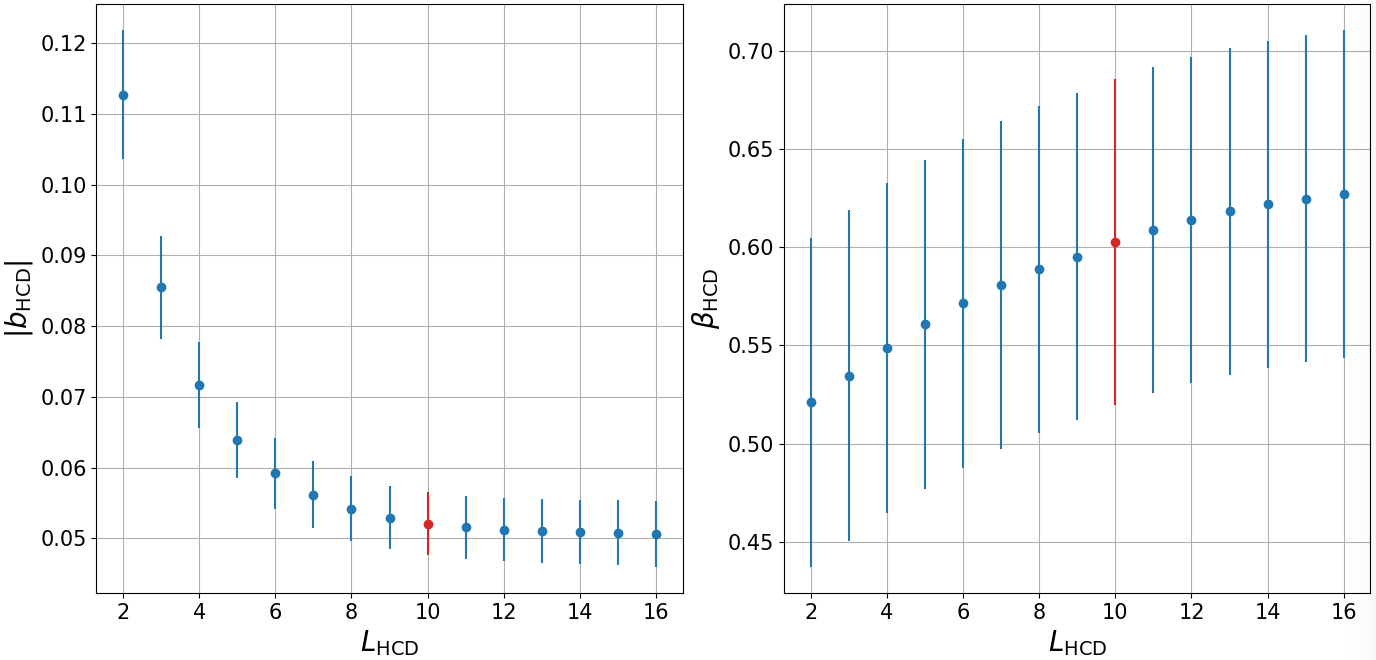
\includegraphics[scale=0.4]{bias_hcd_vs_L0_dr16}
  \caption{Evolution des mesures des paramètres $b_{\textsc{HCD}}$ et $\beta_{\textsc{HCD}}$ en fonction de la valeur $L_{\textsc{HCD}}$ choisie pour l'ajustement.
    % Les mesures sont faites sur l'auto-corrélation \lya{}$\times$\lya{} estimée à partir de \Nmocks{} réalisations des mocks eboss-0.2 et moyennée sur les 4 bins en redshift.}
    Les mesures sont faites sur l'auto-corrélation \lya{}$\times$\lya{} estimée à partir des données DR16 et moyennée sur les quatre bins en redshift.
    }
  \label{fig:bias_hcd_vs_L0_dr16}
\end{figure}
\begin{figure}
  \centering
  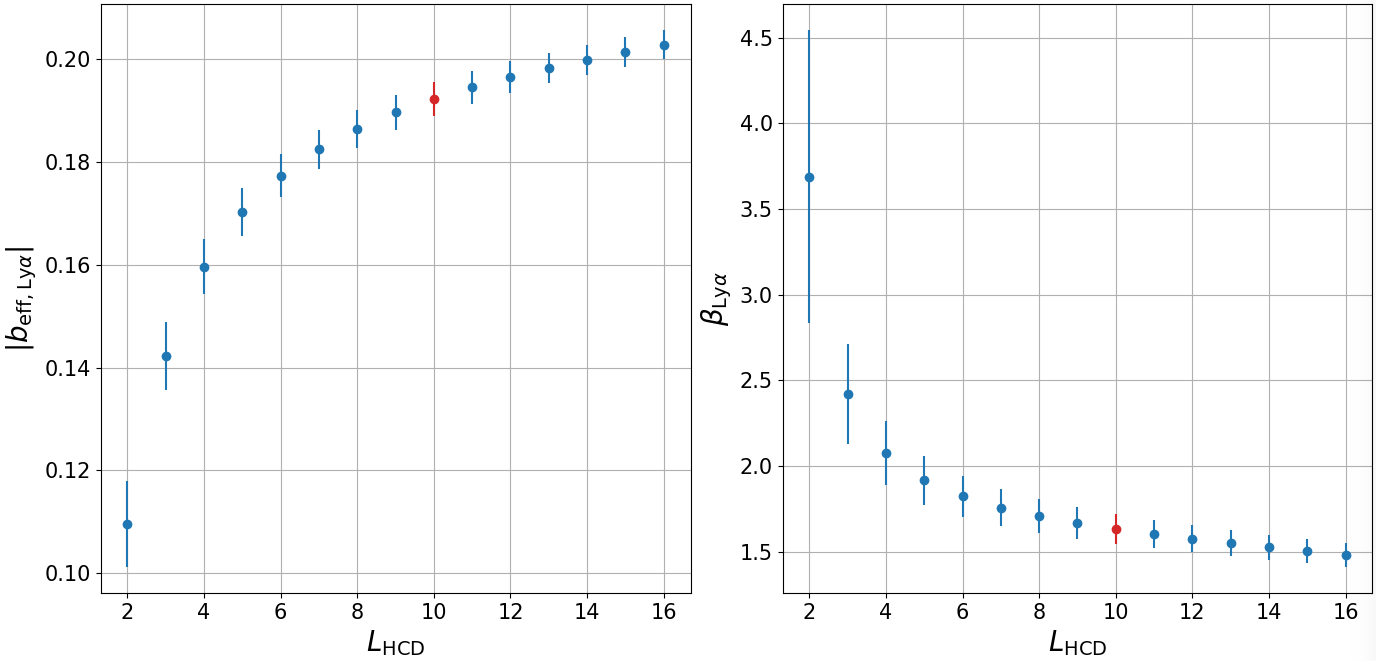
\includegraphics[scale=0.45]{bias_lya_vs_L0_dr16}
  \caption{Evolution des mesures des paramètres $b_{\mathrm{eff},\mathrm{Ly}\alpha}$ et $\beta_{\mathrm{Ly}\alpha}$ en fonction de la valeur $L_{\textsc{HCD}}$ choisie pour l'ajustement.
    % Les mesures sont faites sur l'auto-corrélation \lya{}$\times$\lya{} estimée à partir de \Nmocks{} réalisations des mocks eboss-0.2 et moyennée sur les 4 bins en redshift. La ligne horizontale bleue donne la mesure faite sur les \Nmocks réalisations des mocks eboss-0.0. Les lignes tiretées donnent les erreurs à $1 \sigma$.}
    Les mesures sont faites sur l'auto-corrélation \lya{}$\times$\lya{} estimée à partir des données DR16 et moyennée sur les quatre bins en redshift.
    }
  \label{fig:bias_lya_vs_L0_dr16}
\end{figure}


\section{Etude de la modélisation des HCD}
\label{sec:etude_model_hcd}
% Suite aux différents points énoncés dans la section précédente, nous avons mené une analyse sur les mocks, afin de mieux comprendre la modélisation des HCD, et d'essayer d'identifier les potentielles systématiques qui affectent la mesure des paramètres \lya{}.
Suite aux différents points énoncés dans la section précédente, nous avons étudié l'effet qu'ont les HCD sur les paramètres \lya{} mesurés dans les mocks.
En effet, les mocks sont l'outil parfait pour ce genre d'analyse : ils permettent, contrairement aux données, de connaître la quantité de \lya{} présente, et de comparer cette quantité à ce qui est mesuré par l'ajustement. De plus, nous connaissons le nombre et les distributions en redshift ($z$) et en densité de colonne ($\log n_{\mathrm{HI}}$) des HCD ajoutés dans les mocks, ce qui n'est pas le cas des données.
Dans cette section, nous comparons les paramètres \lya{} mesurés dans les mocks sans HCD (raw mocks, eboss-0.0) et avec HCD (eboss-0.2). Nous comparons aussi les paramètres \lya{} mesurés en utilisant différentes modélisations des HCD.

\subsection{Comparaison des mocks}
\label{subsec:comparaison_mocks}
Comme expliqué dans le chapitre~\ref{chap:mock_ana}, nous avons analysé \Nmocks{} réalisations des raw mocks, des mocks eboss-0.0 et des mocks eboss-0.2.
Dans chacun des cas, nous ajustons le modèle sur $20 < r < \SI{180}{\perh\Mpc}$ et mesurons les paramètres \lya{}.
La figure~\ref{fig:bias_cf} présente les mesures de ces paramètres dans chaque bin en redshift pour chacune des versions des mocks.
Nous pouvons remarquer que les valeurs des paramètres \lya{} mesurés changent selon la version des mocks.
Les paramètres mesurés dans les raw mocks sont très proches des paramètres visés, mesurés dans les données DR16. Ceci montre que la procédure d'ajustement des paramètres des mocks que nous avons mise en place est efficace pour obtenir les bons $b_{\mathrm{eff},\mathrm{Ly}\alpha}$ et $\beta_{\mathrm{Ly}\alpha}$.

Lorsque nous comparons maintenant les valeurs de $b_{\mathrm{eff},\mathrm{Ly}\alpha}$ et $\beta_{\mathrm{Ly}\alpha}$ mesurées dans les raw mocks à celles mesurées dans les mocks eboss-0.0, nous observons un écart statistiquement significatif.
L'effet sur $\beta_{\mathrm{Ly}\alpha}$ est faible, et les valeurs de $\beta_{\mathrm{Ly}\alpha}$ mesurées dans les mocks eboss-0.0 restent compatibles avec les données DR16.
Cependant, l'effet sur le biais effectif $b_{\mathrm{eff},\mathrm{Ly}\alpha}$ est important (de l'ordre de \SI{10}{\percent}) et statistiquement significatif.
% Cela implique que l'ajout du continuum et du bruit par quickquasars, l'ajustement du continuum ou la prise en compte des effets liés à cet ajustement par la matrice de distorsion affecte la mesure de $b_{\mathrm{eff},\mathrm{Ly}\alpha}$ et $\beta_{\mathrm{Ly}\alpha}$. Nous suspectons la matrice de distorsion de ne pas capturer tous les effets produits par l'ajustement du continuum, ce qui pourrait expliquer l'écart entre les raw mocks et les mocks eboss-0.0.
% Il semble que la matrice de distorsion ne prenne pas totalement en compte l'ajout du continuum et du bruit par \texttt{quickquasars} et l'ajustement du continuum dans l'analyse.
Les écarts observés sont attribués à la matrice de distorsion, qui ne capture pas l'intégralité des distorsions produites par l'ajustement du continuum.
La figure~\ref{fig:dmat_effect} présente la comparaison des mocks eboss-0.0, en rouge, avec les mocks eboss-raw multipliés par la matrice de distorsion, en vert. Si la matrice de distorsion était parfaite, les courbes rouge et verte seraient confondues, ce qui n'est pas le cas. Une étude approfondie de la matrice de distorsion et de l'ajout du continuum par \texttt{quickquasars} est nécessaire pour comprendre ces différences.
\begin{figure}
  \centering
  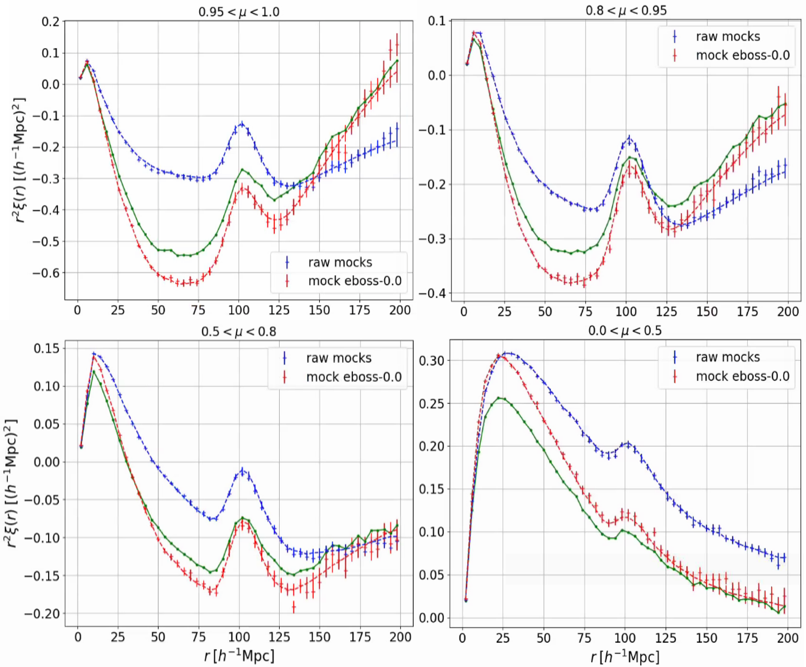
\includegraphics[scale=0.5]{dmat_effect}
  \caption{Fonction de corrélation \lya{}$\times$\lya{} estimée à partir des mocks eboss-raw, en bleu, et des mocks eboss-0.0, en rouge. Les fonctions de corrélation sont estimées à partir de 30 réalisations des mocks. La courbe verte correspond à la corrélation \lya{}$\times$\lya{} estimée à partir des mocks eboss-raw et multipliée par la matrice de distorsion.}
  \label{fig:dmat_effect}
\end{figure}

Enfin, nous observons un écart entre les valeurs de $b_{\mathrm{eff},\mathrm{Ly}\alpha}$ et $\beta_{\mathrm{Ly}\alpha}$ mesurées dans les mocks eboss-0.0 et eboss-0.2. L'écart mesuré pour $b_{\mathrm{eff},\mathrm{Ly}\alpha}$ est comparable à celui mesuré entre les mocks eboss-0.0 et les raw mocks.
L'écart mesuré sur $\beta_{\mathrm{Ly}\alpha}$ est plus important. Les valeurs obtenues dans l'ajustement des mocks eboss-0.2 ne sont pas compatibles avec celles mesurées dans les données DR16.
% Nous suspectons les HCD d'être à l'origine de cet écart. Comme expliqué dans la section~\ref{subsec:stab_pars_lya}, les paramètres \lya{} sont très corrélés avec ceux des HCD. Nous aurions pu par exemple choisir un $L_{\textsc{HCD}}$ plus faible dans l'ajustement des mocks eboss-0.2, ce qui aurait permis d'avoir des mesures compatibles de $\beta_{\mathrm{Ly}\alpha}$ entre les mocks eboss-0.0 et eboss-0.2 (voir figure~\ref{fig:bias_lya_vs_L0}).
Comme expliqué dans la section~\ref{subsec:stab_pars_lya}, les paramètres \lya{} sont très corrélés avec ceux des HCD, en particulier avec $L_{\textsc{HCD}}$ qui est fixé à \SI{10}{\perh\Mpc}.
Nous regardons dans un premier temps la corrélation des paramètres \lya{} avec $L_{\textsc{HCD}}$ dans les mocks. La figure~\ref{fig:bias_lya_vs_L0} présente la mesure de $b_{\mathrm{eff},\mathrm{Ly}\alpha}$ et $\beta_{\mathrm{Ly}\alpha}$ dans les mocks-0.2 pour différentes valeurs de $L_{\textsc{HCD}}$. Le corrélation avec $L_{\textsc{HCD}}$ est similaire à celle observée dans les données (figure~\ref{fig:bias_lya_vs_L0_dr16}).
Cette figure suggère qu'il faut utiliser une valeur de $L_{\textsc{HCD}}$ entre 2 et \SI{4}{\perh\Mpc} afin d'obtenir une mesure des paramètres \lya{} en accord avec les mocks eboss-0.0.
Ainsi nous produisons un ajustement des mocks eboss-0.2 avec $L_{\textsc{HCD}} = \SI{2.8}{\perh\Mpc}$ (le choix de cette valeur particulière est expliquée dans la section~\ref{subsec:comprendre_hcd}).
Le résultat de cet ajustement est présenté dans le tableau~\ref{tab:cf_eboss02_L028}.
% Les paramètres \lya{} obtenus sont en bien meilleur accord avec les mocks eboss-0.2 que lorsque nous utilisons $L_{\textsc{HCD}} = \SI{10}{\perh\Mpc}$.
Les paramètres \lya{} obtenus sont maintenant compatibles à $\num{1.2} \sigma$ et $\num{1.3} \sigma$  avec les mocks eboss-0.0.
% Ceci suggère que la valeur de $L_{\textsc{HCD}}$ utilisée dans l'ajustement des données DR16 est mal choisi, ou que les distributions de HCD entre les mocks et les données sont significativement différentes. Nous investigons le choix de $L_{\textsc{HCD}}$ dans la section~\ref{subsec:comprendre_hcd}.
Ceci suggère que la valeur de $L_{\textsc{HCD}}$ utilisée dans l'ajustement des données DR16 est mal choisie. Nous investigons le choix de $L_{\textsc{HCD}}$ dans la section~\ref{subsec:comprendre_hcd}.
% Aussi, nous remarquons que le biais du \lya{} préfèrerait une valeur de $L_{\textsc{HCD}}$ légèrement plus grande, tandis que $\beta_{\mathrm{Ly}\alpha}$ préfèrerait une valeur légèrement plus faible. Ceci indique que le modèle utilisé pour modéliser les HCD n'est pas parfait.}

\begin{figure}
  \centering
  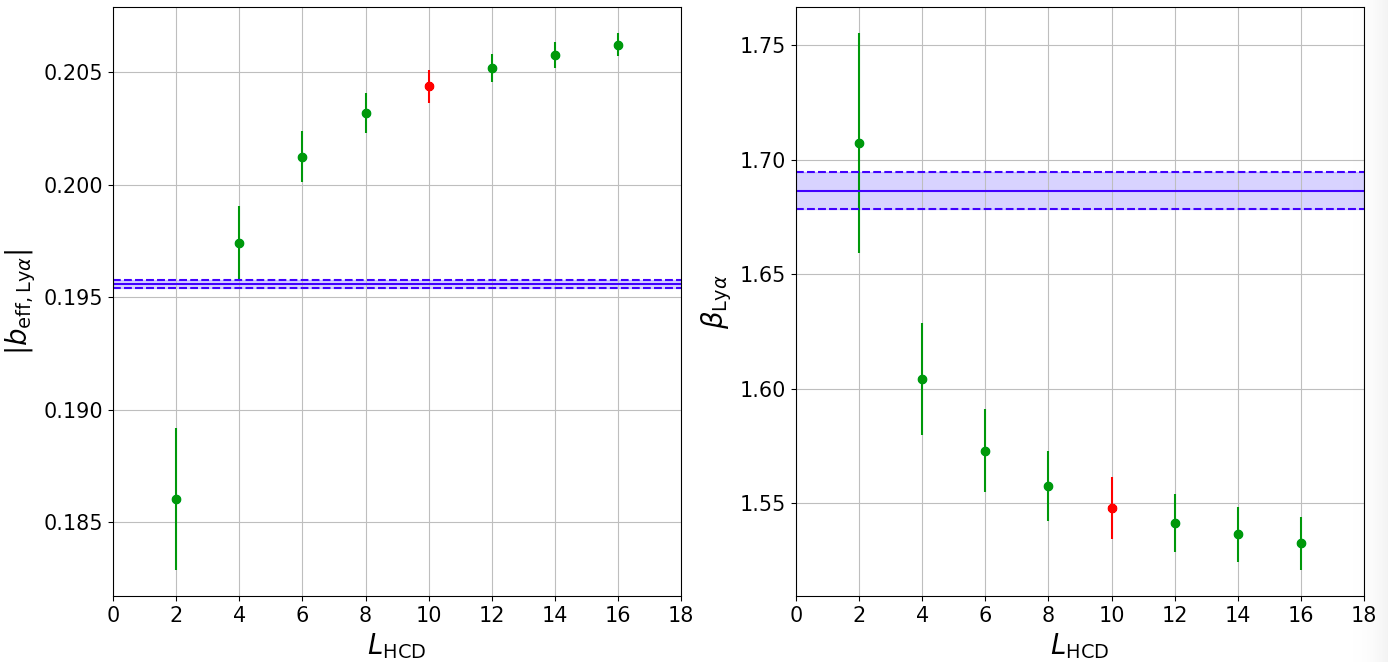
\includegraphics[scale=0.33]{bias_lya_vs_L0}
  \caption{Evolution des mesures des paramètres $b_{\mathrm{eff},\mathrm{Ly}\alpha}$ et $\beta_{\mathrm{Ly}\alpha}$ en fonction de la valeur $L_{\textsc{HCD}}$ choisie pour l'ajustement.
    Les mesures sont faites sur l'auto-corrélation \lya{}$\times$\lya{} estimée à partir de \Nmocks{} réalisations des mocks eboss-0.2 et moyennée sur les 4 bins en redshift. La ligne horizontale bleue donne la mesure faite sur les \Nmocks{} réalisations des mocks eboss-0.0. Les lignes tiretées bleues donnent les erreurs à $1 \sigma$.}
  \label{fig:bias_lya_vs_L0}
\end{figure}

\begin{table}[]
  \centering
  \caption{Résultats des ajustements de l'auto-corrélation \lya{}$\times$\lya{} estimée sur \Nmocks{} réalisations des mocks et moyennée sur les quatre bins en redshift. La première ligne donne l'ajustement des mocks eboss-0.0. La deuxième donne l'ajustement des mocks eboss-0.2 comme décrit dans la section~\ref{subsec:model_mock}. La troisième ligne donne le même ajustement que la deuxième mais en utilisant $L_{\textsc{HCD}} = \SI{2.8}{\perh\Mpc}$.}
  \label{tab:cf_eboss02_L028}
  \footnotesize
  \begin{tabular}{ccccccc}
    \toprule
    % \myalign{c}{version} & \myalign{c}{$b_{\mathrm{eff},\mathrm{Ly}\alpha}$} & \myalign{c}{$\beta_{\mathrm{Ly}\alpha}$} & \myalign{c}{$b_{\textsc{HCD}}$} & \myalign{c}{$\beta_{\textsc{HCD}}$} & \myalign{c}{$L_{\textsc{HCD}}\;[\si{\perh\Mpc}]$} & \myalign{c}{$\chi^2 \; (n_{dof})$} \\
    version & $b_{\mathrm{eff},\mathrm{Ly}\alpha}$ & $\beta_{\mathrm{Ly}\alpha}$ & $b_{\textsc{HCD}}$ & $\beta_{\textsc{HCD}}$ & $L_{\textsc{HCD}}\;[\si{\perh\Mpc}]$ & $\chi^2 \; (n_{dof})$ \\
    \midrule
    eboss-0.0 & $-0.1956 \pm 0.0002$ & $1.687 \pm 0.008$ & & & & 1562 (1570) \\
    eboss-0.2 & $-0.2044 \pm 0.0007$ & $1.548 \pm 0.014$ & $-0.0080 \pm 0.0010$ & $0.487 \pm 0.089$ & $10$ & 1573 (1568) \\
    eboss-0.2 & $-0.1925 \pm 0.0023$ & $ 1.647 \pm 0.034$ &  $-0.0177 \pm 0.0025$ & $ 0.455 \pm 0.090$ & $2.8$ & 1578 (1568) \\ 
    \bottomrule
  \end{tabular}
\end{table}

% Dans un premier temps, nous étudions si en changeant $L_{\textsc{HCD}}$, nous obtenons des mesures des paramètres \lya{} compatibles dans les mocks eboss-0.0 et eboss-0.2.
% Pour ce faire, nous ajustons la corrélation \lya{}$\times$\lya{} estimée à partir des \Nmocks{} réalisations des mocks eboss-0.2 et moyennée dans les quatre bins en redshift.
% Cet ajustement est fait en fixant les paramètres \lya{} aux valeurs obtenues lors de l'ajustement des mocks eboss-0.0 et en laissant libre le paramètre $L_{\textsc{HCD}}$.
% Puis dans un second temps, nous ajustons de nouveau les mocks eboss-0.2 en utilisant la valeur de $L_{\textsc{HCD}}$ obtenue avec l'ajustement précédent.
% Le tableau~\ref{tab:cf_eboss02_L0free} résume les résultats de ces ajustements.
% Comme le suggère la figure~\ref{fig:bias_lya_vs_L0}, la valeur de $L_{\textsc{HCD}}$ obtenue dans l'ajustement des mocks eboss-0.2 avec les paramètres lya{} fixés est plus faible que \SI{10}{\perh\Mpc}. Réduire cette valeur permet d'obtenir un biais \lya{} plus faible et un paramètre RSD \lya{} plus grand.
% Cependant, lorsque nous relâchons les paramètres \lya{} et utilisons $L_{\textsc{HCD}} = \SI{4.38}{\perh\Mpc}$, les paramètres \lya{} que nous obtenons ne sont toujours pas en accord avec ceux mesurés dans les mocks eboss-0.0.
% En effet, l'ajustement fait avec les paramètres \lya{} fixés préfère une valeur de $\beta_{\textsc{HCD}}$ plus faible pour compenser la valeur plus importante de $\beta_{\mathrm{Ly}\alpha}$.
% Nous avons esayé de produire un autre ajustement dans lequel, en plus des paramètres \lya{}, nous fixons $\beta_{\textsc{HCD}} = \num{0.487}$. Mais lorsque nous relâchons ces paramètres et utilisons la nouvelle valeur de $L_{\textsc{HCD}}$ obtenue, le problème se déplace sur $b_{\textsc{HCD}}$.
% Ainsi, nous n'arrivons pas à produire un ajustement des mocks eboss-0.2 dans lequel les mesures des paramètres \lya{} sont en accord avec les mesures faites sur les mocks eboss-0.0.

% \begin{table}[]
%   \centering
%   \caption{Résultats des ajustements de l'auto-corrélation \lya{}$\times$\lya{} estimée sur \Nmocks réalisations des mocks et moyennée sur les quatre bins en redshift. La première ligne donne l'ajustement des mocks eboss-0.0. La deuxième donne l'ajustement des mocks eboss-0.2 comme décrit dans la section~\ref{subsec:model_mock}. La troisième ligne donne le même ajustement que la deuxième mais avec les paramètres \lya{} fixés et $L_{\textsc{HCD}}$ libre. Enfin la dernière ligne donne le même ajustement que la deuxième mais en utilisant la valeur de $L_{\textsc{HCD}}$ obtenue dans l'ajustement de la troisième ligne. Le paramètre $L_{\textsc{HCD}}$ est donné en \si{\perh\Mpc}.}
%   \label{tab:cf_eboss02_L0free}
%   \scriptsize
%   \begin{tabular}{lllllll}
%     \toprule
%     \myalign{c}{version} & \myalign{c}{$b_{\mathrm{eff},\mathrm{Ly}\alpha}$} & \myalign{c}{$\beta_{\mathrm{Ly}\alpha}$} & \myalign{c}{$b_{\textsc{HCD}}$} & \myalign{c}{$\beta_{\textsc{HCD}}$} & \myalign{c}{$L_{\textsc{HCD}}$} & \myalign{c}{$\chi^2 \; (n_{dof})$} \\
%     \midrule
%     eboss-0.0 & $-0.1956 \pm 0.0002$ & $1.687 \pm 0.008$ & & & & 1562 (1570) \\
%     eboss-0.2 & $-0.2044 \pm 0.0007$ & $1.548 \pm 0.014$ & $-0.0080 \pm 0.0010$ & $0.487 \pm 0.089$ & $10$ & 1573 (1568) \\
%     eboss-0.2 \& \lya{} fixé & $-0.1956$ & $1.687$ & $-0.0174 \pm 0.0005$ & $0.174 \pm 0.048$ & $4.38 \pm 0.47$ & 1591 (1569) \\
%     eboss-0.2 \& $L_{\textsc{HCD}} = 4.38$ & $-0.1984 \pm 0.0015$ & $ 1.596 \pm 0.023$ &  $-0.0127 \pm 0.0017$ & $ 0.464 \pm 0.089$ & $4.38$ & 1576 (1568) \\ 
%     \bottomrule
%   \end{tabular}
% \end{table}




\subsection{Effet du masquage des HCD}
\label{subsec:effet_masquage_hcd}
Dans l'analyse des mocks eboss-0.2, comme pour les données, les HCD pour lesquels $\log n_{\textsc{HI}} > \num{20.3}$ sont masqués lors du calcul des $\delta_F$.
Comme expliqué dans la section~\ref{subsec:stab_pars_lya}, le masquage des HCD dans les données s'effectue selon le résultat de l'agorithme d'identification. Les HCD identifiés puis reconstruits avec $\log n_{\textsc{HI}} > \num{20.3}$ sont masqués. Dans le cas des mocks, les HCD avec $\log n_{\textsc{HI}} > \num{20.3}$ sont masqués à partir du \og vrai \fg catalogue. Nous étudions ici l'effet du masquage à partir du catalogue produit par l'algorithme d'identification.
Pour ce faire, nous produisons l'analyse d'une réalisation de mock eboss-0.2, pour laquelle nous utilisons l'algorithme d'identification pour créer un catalogue de HCD. Le champ $\delta_F$ est calculé en masquant les HCD identifiés par l'algorithme, puis la fonction de corrélation \lya{}$\times$\lya{} est estimée dans les quatre bins en redshift utilisés jusqu'ici. Nous nommons cette analyse \emph{eboss-0.2\_finder}.
La figure~\ref{fig:cf_finder_vs_true} présente la fonction de corrélation \lya{}$\times$\lya{} estimée à partir de la même réalisation des mocks, en version eboss-0.0, eboss-0.2 et eboss-0.2\_finder.
Les fonctions de corrélation affichées sont la moyenne des fonctions de corrélation estimées dans les quatre bins en redshift.
Dans les trois versions, le code \texttt{quickquasars} utilise les mêmes quasars pour produire les spectres synthétiques, et ajoute le même bruit à ces spectres dans les trois cas. Ceci nous permet d'avoir les mêmes fluctuations statistiques dans le calcul de la corrélation \lya{}$\times$\lya{}, et ainsi d'avoir des mesures de biais comparables.
L'effet des HCD (avec une densité de colonne $\num{17.2} < \log n_{\textsc{HI}} < \num{20.3}$) est visible en comparant la corrélation montrée en rouge à celle montrée en bleu. Comme expliqué dans la section~\ref{subsec:model_donnees}, l'effet principal des HCD est d'augmenter le biais effectif.
Par ailleurs, le fait que l'effet des HCD soit légèrement plus important sur la corrélation de la version eboss-0.2 que sur celle de la version  eboss-0.2\_finder suggère que l'algorithme identifie correctement les HCD pour lesquels $\log n_{\textsc{HI}} > \num{20.3}$, et identifie une petite partie des HCD avec $\log n_{\textsc{HI}} < \num{20.3}$ et les reconstruit avec $\log n_{\textsc{HI}} > \num{20.3}$. Ceci a pour effet de masquer des HCD qui ne possèdent pas une densité de colonne supérieure à \num{20.3}.
Ceci est confirmé par la figure~\ref{fig:nhi_finder}, qui compare la densité de colonne $\log n_{\textsc{HI}}$ trouvée par le finder (output) à la \og vrai \fg densité de colonne des HCD des mocks (input). Nous voyons sur cette figure que l'algorithme a tendance à surestimer la densité de colonne $\log n_{\textsc{HI}}$, ce qui est en accord avec nos observations.
Notons par ailleurs que l'algorithme d'identification possède une efficacité de \SI{90}{\percent} pour $\log n_{\textsc{HI}} > \num{20.3}$. L'effet de ces HCD non identifiés avec $\log n_{\textsc{HI}} > \num{20.3}$ est donc plus faible que l'effet des HCD dont le $\log n_{\textsc{HI}}$ est surestimé.
  Ceci s'explique par le faible nombre de HCD avec $\log n_{\textsc{HI}} > \num{20.3}$.


\begin{figure}
  \centering
  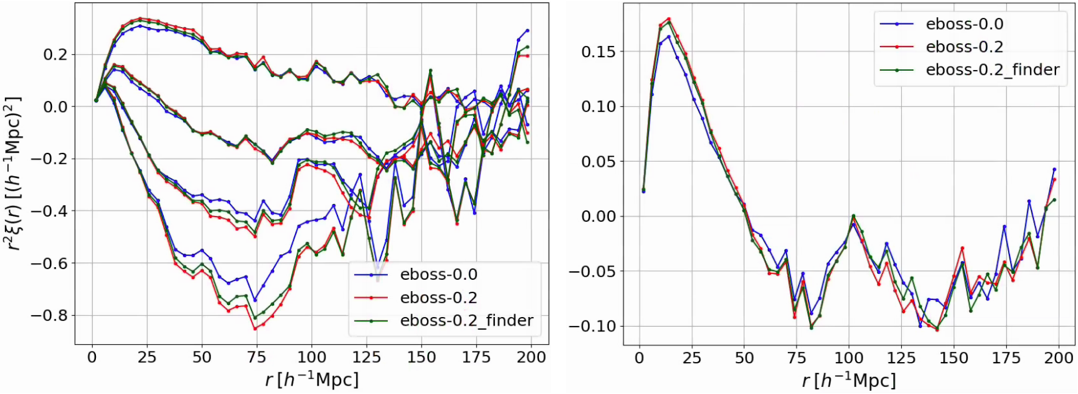
\includegraphics[scale=0.4]{cf_finder_vs_true}
  \caption{Fonctions de corrélation \lya{}$\times$\lya{} estimées à partir d'une réalisation des mocks eboss-0.0 (bleu), eboss-0.2 (rouge) et eboss-0.2\_finder (vert). La version eboss-0.2\_finder correspond aux mocks eboss-0.2, dans lesquels les HCD ont été masqués en utilisant le catalogue de HCD produit par l'algorithme d'identification.
    Le graphique de gauche montre les corrélations dans quatre gammes en $\mu$. Ces gammes sont, de haut en bas : $\num{0} < \mu < \num{0.5}$, $\num{0.5} < \mu < \num{0.8}$, $\num{0.8} < \mu < \num{0.95}$ et $\num{0.95} < \mu < \num{1}$. Le graphique de droite montre les corrélations moyennées sur $\num{0}  < \mu < \num{1}$.}
  \label{fig:cf_finder_vs_true}
\end{figure}

Le tableau~\ref{tab:finder_vs_true} donne les résultats des ajustements des trois corrélations présentées sur la figure~\ref{fig:cf_finder_vs_true}. La statistique d'une seule réalisation n'est pas suffisante pour identifier des potentielles systématiques. Cependant, la précision de la mesure des paramètres \lya{} dans les données DR16 étant comparable à celle des mocks eboss-0.2, les potentielles systématiques sont inférieures à l'erreur statistique sur cette mesure.
Il serait tout de même intéressant de mener cette étude sur un plus grand nombre de réalisations.


\begin{table}[]
  \centering
  \caption{Résultat de l'ajustement de la corrélation \lya{}$\times$\lya{} estimée à partir d'une réalisation des mocks eboss-0.0, eboss-0.2 et eboss-0.2\_finder. La version eboss-0.2\_finder correspond aux mocks eboss-0.2, dans lesquels les HCD ont été masqués en utilisant le catalogue de HCD produit par l'algorithme d'identification.}
  \label{tab:finder_vs_true}
  \begin{tabular}{lllll}
    \toprule
    \myalign{c}{version} & \myalign{c}{$b_{\mathrm{eff},\mathrm{Ly}\alpha}$} & \myalign{c}{$\beta_{\mathrm{Ly}\alpha}$} & \myalign{c}{$b_{\textsc{HCD}}$} & \myalign{c}{$\beta_{\textsc{HCD}}$} \\
    \midrule
    eboss-0.0 & $-0.1970 \pm 0.0009$ & $ 1.641 \pm 0.039$ & & \\
    eboss-0.2 & $-0.1979 \pm 0.0038$ & $1.578 \pm 0.069$ & $-0.0201 \pm 0.0053$ & $0.499 \pm 0.090$ \\
    eboss-0.2\_finder & $-0.1951 \pm 0.0039$ & $1.592 \pm 0.074$ & $-0.0186 \pm 0.0054$ & $0.494 \pm 0.091$ \\
    \bottomrule
  \end{tabular}
\end{table}

\begin{figure}
  \centering
  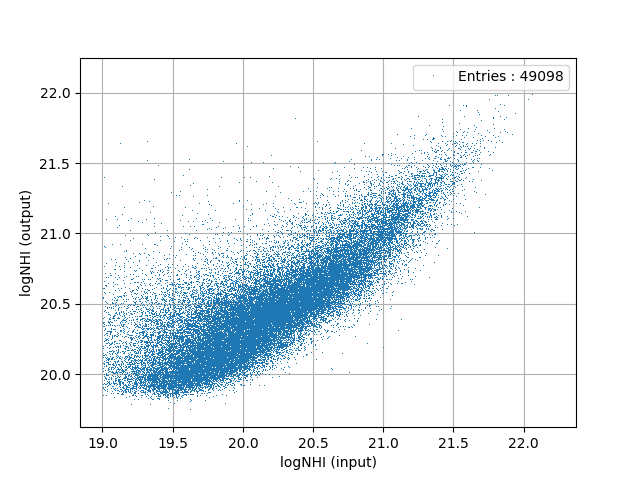
\includegraphics[scale=0.8]{nhi_finder.png}
  \caption{Densité de colonne $\log n_{\textsc{HI}}$ trouvée par le finder (logNHI output) en fonction de la \og vrai \fg densité de colonne des HCD des mocks (logNHI input). Cette comparaison est produite par Jim Rich et Solène Chabannier, du groupe cosmologie du CEA, à l'aide des mocks (Chabanier et al. (in prep)).}
  \label{fig:nhi_finder}
\end{figure}

\subsection{Une meilleure modélisation des HCD}
\label{subsec:model_alter_hcd}
% Dans le but de tester la modélisation des HCD, nous avons ajustés les mocks et les données en utilisant une modélisation différente des HCD.
Toujours dans l'optique de tester la robustesse de la mesure des paramètres \lya{}, nous avons utilisé une modélisation des HCD différente de celle décrite dans la section~\ref{subsec:model_donnees} et utilisée jusqu'ici pour modéliser les mocks et les données.
Ce modèle est développé par Edmond Chaussidon et Julien Guy, au sein du groupe \lya{} de la collaboration DESI.
Nous faisons référence à ce modèle via le nom \emph{modèle C-G}. Le modèle des HCD décrit dans la section~\ref{subsec:model_donnees} est dénommé \emph{modèle de Rogers}.
% Ce modèle, contrairement au modèle décrit dans la section~\ref{subsec:model_donnees}, ne masque pas les HCD identifiés par l'algorithme et vérifiant $\log n_{\textsc{HI}} > 20.3$.
% Ce choix est fait dans le but de s'affranchir des potentiels systématiques produites par l'utilisation de l'algorithme de détection.
% Ainsi, le modèle C-G prend en compte les effets sur les corrélations \lya{}$\times$\lya{} et \lya{}$\times$QSO produits par l'ensemble des HCD dans les données.
% Pour ce faire, 
Le modèle C-G, contrairement au modèle de Rogers, n'a pas besoin de masquer les HCD identifiés par l'algorithme. Il prend en compte les effets sur les corrélations \lya{}$\times$\lya{} et \lya{}$\times$QSO produits par l'ensemble des HCD dans les données.
% La modélisation définie dans l'équation~\ref{eq:bias_hcd_def} est aussi utilisée, mais plutôt que de définir $F_{\textsc{HCD}}$ comme une fonction exponentielle avec une paramètre $L_{\textsc{HCD}}$ qui reflète la taille caractéristique des HCD présents dans les données (équation~\ref{eq:f_hcd_def}),
Les deux modèles utilisent la modélisation définie dans l'équation~\ref{eq:bias_hcd_def}.
Cependant, dans le cas du modèle C-G, plutôt que de définir $F_{\textsc{HCD}}$ comme une fonction exponentielle avec un paramètre effectif $L_{\textsc{HCD}}$ qui reflète la taille caractéristique des HCD non masqués (équation~\ref{eq:f_hcd_def}),
% la fonction $F_{\textsc{HCD}}$ qui est utilisée correspond au profil de Voigt résultant de la distribution en $\log n_{\textsc{HI}}$ des HCD présents dans les données.
la fonction $F_{\textsc{HCD}}$ est calculée en prenant en compte la distribution en $\log n_{\textsc{HI}}$ des HCD présents dans les données.
% le modèle calcule le profil de Voigt résultant de la distribution des HCD présent. La fonction $F_{\textsc{HCD}}$ est choisie comme étant égale à ce profil de Voigt ainsi calculé.
% la fonction $F_{\textsc{HCD}}$ qui est utilisée par le modèle C-G correspond au profil de Voigt résultant de la distribution en $\log n_{\textsc{HI}}$ des HCD présents dans les données.
L'avantage de cette méthode est qu'elle n'utilise pas le paramètre effectif $L_{\textsc{HCD}}$. Elle permet donc de modéliser des distributions de HCD avec une plus grande gamme en $\log n_{\textsc{HI}}$, là où le modèle de Rogers, utilisé pour analyser les données DR16, ne fonctionne plus très bien.
De plus, le modèle C-G permet de s'affranchir des potentiels systématiques induites par l'utilisation de l'algorithme de détection.
Cependant, afin de calculer le terme $F_{\textsc{HCD}}$ correspondant à la distribution de HCD présents, nous devons justement connaître cette distribution. Si cela est possible pour les mocks, cela ne l'est pas pour les données, car nous ignorons la distribution en $\log n_{\textsc{HI}}$ des HCD non identifiés, c'est à dire pour lesquels $\log n_{\textsc{HI}} < \num{20.3}$.
Ainsi, lorsque nous analysons les données DR16 avec le modèle C-G, nous supposons que la distribution de HCD dans les données est celle du modèle \texttt{pyigm}, utilisée dans les mocks. % la même que celle des mocks. Nous utilisons donc le même profil de Voigt.

Du fait que, pour le modèle C-G, le terme $F_{\textsc{HCD}}$ soit calculé à partir de la distribution en $\log n_{\textsc{HI}}$ des HCD présents, nous pouvons envisager d'ajuster avec ce modèle, des mocks avec différentes distributions de HCD : les mocks eboss-0.2 où les HCD avec $\log n_{\textsc{HI}} < \num{20.3}$ sont  masqués, les mocks eboss-0.2 où tous les HCD sont présents ($\num{17.2} < \log n_{\textsc{HI}} < \num{22.5}$), ou n'importe quelle autre distribution.

\paragraph{}
Afin de tester le modèle C-G, et de le comparer au modèle de Rogers, nous vérifions premièrement que ces deux modèles, lorsqu'ils sont ajustés sur les mocks eboss-0.0, mesurent une quantité de HCD compatible avec 0.

Par ailleurs, dans une étude préliminaire au choix des paramètres \lya{} à utiliser pour construire les mocks, nous étudions comment ces deux modèles se comportent lorsque nous triplons la quantité de HCD dans les mocks.
% Pour ce faire, nous avons produit deux réalisations eboss-0.2, dont l'une posséde trois fois plus de HCD que l'autre.
Pour ce faire, à partir d'une même réalisation des mocks, nous produisons deux versions de quickquasars eboss-0.2 : l'une avec le catalogue de HCD standard, l'autre avec un catalogue contenant 3 fois plus de HCD. Dans ces deux versions, les HCD qui vérifient $\log n_{\mathrm{HI}} > \num{20.3}$ sont masqués. Afin de faciliter la comparaison des résultats, nous utilisons le même sous-échantillon de quasars et ajoutons le même bruit pour produire les spectres synthétiques puis calculer la corrélation \lya{}$\times$\lya{} à partir de ces deux versions.
Puis, nous ajustons la fonction de corrélation \lya{}$\times$\lya{}, estimées à partir de ces deux versions, avec le modèle de Rogers et le modèle C-G. Le paramètre $b_{\textsc{HCD}} $ étant proportionnel au nombre de HCD, nous nous attendons à mesurer un biais trois fois plus grand dans la réalisation possédant trois fois plus de HCD.
Cependant, ce n'est pas ce que nous observons. Le tableau~\ref{tab:hcd_dndz3} résume ces mesures.
Pour une même version, les mesures de $b_{\textsc{HCD}}$ faites avec le modèle de Rogers ou le modèle C-G ne sont pas compatibles.
Comme nous le verrons dans la section~\ref{subsec:comprendre_hcd}, cela est dû à la valeur de $L_{\textsc{HCD}}$ mal choisie pour le modèle de Rogers.
De plus, pour un même modèle, nous remarquons que $b_{\textsc{HCD}}$  mesuré dans la version contenant 3 fois plus de HCD n'est pas compatible avec 3 fois le biais des HCD mesuré dans l'autre version. Le biais des HCD mesuré dans la version contenant 3 fois plus de HCD est sous-estimé.
Ceci a pour effet de réduire la mesure de $\beta_{\mathrm{Ly}\alpha}$.
Nous pouvons toute fois noter que le modèle C-G produit des mesures de $b_{\mathrm{eff},\mathrm{Ly}\alpha}$ compatibles dans ces deux versions, ce qui n'est pas le cas du modèle de Rogers.

\begin{table}[]
  \centering
  \caption{Mesures des paramètres $b_{\mathrm{eff},\mathrm{Ly}\alpha}$, $\beta_{\mathrm{Ly}\alpha}$, $b_{\textsc{HCD}}$ et  $\beta_{\textsc{HCD}}$ faites à partir de l'auto-corrélation \lya{}$\times$\lya{} estimée sur une réalisation des mocks eboss-0.2, où les HCD avec $\log n_{\mathrm{HI}} > \num{20.3}$ ont été masqués.
    % Les deux premières lignes donnent les mesures faites avec le modèle de Rogers et le modèle C-G. Les deux dernières lignes donnent les mesures faites avec ces deux modèles en ajustant la corrélation \lya{}$\times$\lya{} estimée sur la même réalisation des mocks mais avec un catalogue contenant 3 fois plus de HCD.}
    % La première section donne les mesures faites avec le modèle de Rogers, et la seconde celles faites avec le modèle C-G.
      Le détail de chaque ajustement est donné dans le texte.}
    \label{tab:hcd_dndz3}
    \small
    \begin{tabular}{lllll}
      \toprule
        \myalign{c}{Version}  & \myalign{c}{$b_{\mathrm{eff},\mathrm{Ly}\alpha}$} & \myalign{c}{$\beta_{\mathrm{Ly}\alpha}$} & \myalign{c}{$b_{\textsc{HCD}}$} & \myalign{c}{$\beta_{\textsc{HCD}}$}  \\
    \midrule
    % modèle Rogers & $-0.1912 \pm 0.0020$ & $1.558 \pm 0.039$ & $-0.0165 \pm 0.0030$ \\
    % modèle C-G & $-0.1708 \pm 0.0058$ & $1.746 \pm 0.095$ & $-0.0323 \pm 0.0062$ \\
    % modèle Rogers \& 3$\times$HCD & $-0.2095 \pm 0.0025$ & $1.295 \pm 0.039$ & $-0.0296 \pm 0.0037$ \\
    % modèle C-G \& 3$\times$HCD & $-0.1713 \pm 0.0071$ & $1.561 \pm 0.110$ & $-0.0598 \pm 0.0077$ \\
     Rogers & $-0.1910\pm 0.0020$ & $1.561 \pm 0.039$ & $-0.0167 \pm 0.0030$ & $0.509 \pm 0.089$ \\
     Rogers \& 3$\times$HCD & $-0.2095 \pm 0.0025$ & $1.295 \pm 0.039$ & $-0.0296 \pm 0.0037$ & $0.514 \pm 0.087$ \\
     Rogers \& 3$\times$HCD \& \lya{} fixé & $-0.1910$ & 	$1.561$ & $-0.0555 \pm 0.0017$ & $0.465 \pm 0.061$ \\
    \midrule
     C-G & $-0.1704 \pm 0.0058$ &	$1.752 \pm 0.096$ & $-0.0327 \pm 0.0062$ & $0.487 \pm 0.089$ \\
     C-G \& 3$\times$HCD & $-0.1713 \pm 0.0071$ & $1.561 \pm 0.110$ & $-0.0598 \pm 0.0077$ & $0.477 \pm 0.087$ \\
     C-G \& 3$\times$HCD \& \lya{} fixé & $ -0.1704$ & $1.752$ &	$-0.0651 \pm 0.0014$ &	$0.277 \pm 0.040$ \\
    \bottomrule
\end{tabular}
\end{table}

Enfin, nous regardons si en fixant les paramètres \lya{}, nous obtenons un biais des HCD compatible avec 3 fois le biais des HCD mesuré dans la version standard. Nous faisons ce test pour le modèle de Rogers et pour le modèle C-G. Le résultat de ces ajustements est donné dans le tableau~\ref{tab:hcd_dndz3} (voir les lignes \og 3$\times$HCD \& \lya{} fixé \fg).
%Similairement aux ajustements présentés dans le tableau~\ref{tab:cf_eboss02_L0free}, fixer les paramètres \lya{} ne résout pas les tensions observées. 
% Pour le modèle de Rogers, le fait de fixer les paramètres \lya{} est compensé par un biais des HCD trop grand. Nous attendons $b_{\textsc{HCD}} = \num{0.0501} \pm \num{0.0090}$ et mesurons $b_{\textsc{HCD}} = -\num{0.0555} \pm \num{0.0017}$. Dans le modèle C-G, c'est le paramètre $\beta_{\textsc{HCD}}$ qui compense les paramètres \lya{} fixés.
% Ainsi, aucun des modèles n'est capable d'identifier correctement les quantités relative de HCD dans deux versions de mocks.
Pour le modèle de Rogers, le fait de fixer les paramètres \lya{} résout bien les tensions obervées : nous attendons $b_{\textsc{HCD}} = \num{0.0501} \pm \num{0.0090}$ et mesurons $b_{\textsc{HCD}} = -\num{0.0555} \pm \num{0.0017}$.
  Cependant, dans le cas du modèle C-G, le paramètre $\beta_{\textsc{HCD}}$ compense les paramètres \lya{} fixés, et la valeur de $b_{\textsc{HCD}}$ obtenue n'est pas compatible avec 3 fois celle mesurée dans la version standard.
  Il serait intéressant de vérifier si en fixant aussi la valeur de $\beta_{\textsc{HCD}}$, nous retrouvons le bon $b_{\textsc{HCD}}$.


\paragraph{}
Afin d'étudier davantage le modèle C-G, nous comparons maintenant la mesure des paramètres \lya{} faite avec ce modèle sur les mocks eboss-0.2 où les HCD avec une densité de colonne $\log n_{\textsc{HI}} > \num{20.3}$ sont masqués, à la mesure faite sur les mocks eboss-0.2 où aucun HCD n'est masqué. Dans chacun des cas, nous utilisons le terme $F_{\textsc{HCD}}$ correspondant à la distribution de HCD considérée.
La comparaison est présentée sur la figure~\ref{fig:bias_cg_rogers_comp}.
\begin{figure}
  \centering
  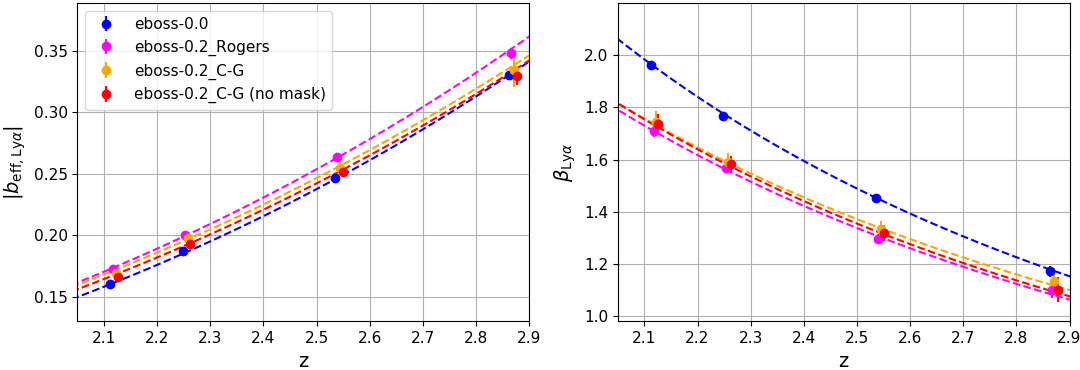
\includegraphics[scale=0.43]{bias_cg_rogers_comp}
  \caption{Mesure des paramètres $b_{\mathrm{eff},\mathrm{Ly}\alpha}$ (gauche) et $\beta_{\mathrm{Ly}\alpha}$ (droite) sur l'auto-corrélation \lya$\times$\lya{} estimée à partir des mocks (30 réalisations utilisées pour chaque mesure). Les points bleus présentent la mesure faite sur les mocks eboss-0.0. Les points magentas la mesure faite sur les mocks eboss-0.2, où les HCD avec $\log n_{\mathrm{HI}} > \num{20.3}$ sont masqués dans le calcul des fonctions de corrélation, et ajustés avec le modèle de Rogers. Les points orange la mesure faite sur ces mêmes fonctions de corrélation, mais ajustées avec le modèle C-G. Enfin, les points rouges présentent la mesure faite sur les mocks eboss-0.2 où aucun HCD n'a été masqué, ajustés avec le modèle C-G.
    Les courbes tiretées correspondent à l'ajustement de chaque jeu de données par une loi de puissance.
Les points bleus sont décalés horizontalement de $\Delta z = -1\times10^{-2}$, les magentas de $\Delta z = -5\times10^{-3}$ et les rouges de $\Delta z = 5\times10^{-3}$ pour des raisons de visibilité.}
  \label{fig:bias_cg_rogers_comp}
\end{figure}
Nous remarquons que la mesure des paramètres \lya{} faite avec le modèle C-G sur les mocks eboss-0.2 où les HCD sont masqués (orange) est compatible avec la mesure faite sur les mocks eboss-0.2 où les HCD ne sont pas masqués (rouge). Ceci est encourageant car cela signifie que le modèle C-G est cohérent avec lui même.
Lorsque nous comparons les mesures faites avec le modèle C-G aux mesures faites avec le modèle de Rogers, nous pouvons identifier une différence statistiquement significative, en particulier pour $b_{\mathrm{eff},\mathrm{Ly}\alpha}$. Nous étudions la cause de ces différences dans la section suivante.
Enfin, les mesures de $b_{\mathrm{eff},\mathrm{Ly}\alpha}$ faites avec le modèle C-G sur les mocks eboss-0.2 sont en meilleur accord avec la mesure faite sur les mocks eboss-0.0 que ne l'est la mesure faite avec le modèle de Rogers sur les mocks eboss-0.2.



\subsection{Mieux comprendre les HCD}
\label{subsec:comprendre_hcd}

\subsubsection{L'effet des HCD sur la fonction de corrélation}
Afin de comprendre pourquoi les deux modèles discutés dans la section précédente ont du mal à distinguer la contribution des HCD de celle du \lya{}, nous avons essayé de comprendre l'effet des HCD sur les fonctions de corrélation.
La figure~\ref{fig:cf_models} présente les différentes composantes du modèle ajusté sur l'auto-corrélation \lya{}$\times$\lya{} estimée à partir des données DR16. Ce modèle est présenté dans la section~\ref{subsec:model_donnees}, il utilise la modélisation de Rogers avec  $L_{\textsc{HCD}} = \SI{10}{\perh\Mpc}$.
% Sur cette figure, la ligne bleue donne le modèle de Kaiser, c'est à dire la fonction de corrélation obtenue à partir du spectre de puissance $P_{\mathrm{QL}}$ (équation~\ref{eq:pk_ql}) et multiplié par le facteur de Kaiser $b_{\mathrm{eff},\mathrm{Ly}\alpha}^2 (1 + \beta_{\mathrm{Ly}\alpha} \mu_k^2)$. La ligne verte donne le modèle de Kaiser multiplié par le terme $F_{\mathrm{NL}}^{\mathrm{auto}}$ qui prend en compte les non-linéarités aux petites échelles. La ligne orange donne le modèle précédent auquel la contribution des HCD a été ajoutée (équation~\ref{eq:bias_hcd_def}). La ligne rouge donne le modèle précédent plus la contribution des métaux et la ligne violette donne le modèle complet. L'auto-corrélation \lya{}$\times$\lya{} estimée à partir des données DR16 est représentée par les points noirs.
La figure~\ref{fig:cf_models_no_dist} donnent ces mêmes composantes non multipliées par la matrice de distorsion.
  En comparant les courbes orange aux courbes vertes, nous pouvons remarquer sur ces figures que l'effet des HCD est assez semblable à celui d'une augmentation du biais.
  Nous pouvons cependant distinguer l'effet des HCD de celui d'une augmentation du biais en regardant le long de la ligne de visée : les HCD ajoutent une corrélation positive pour les petites échelles, et les courbes vertes et jaune ne se coupent pas au niveau de l'axe $y = 0$.
  Ceci est davantage visible lorsque les modèles ne sont pas multipliés par la matrice de distorsion (figure~\ref{fig:cf_models_no_dist}).
  Si nous regardons maintenant la gamme $0 < \mu < \num{0.5}$, l'effet des HCD est très semblable à l'effet d'un facteur multiplicatif appliqué à la courbe verte.
  La distinction entre une augmentation du biais et l'effet des HCD est d'autant plus facile que les modèles utilisent une valeur de $L_{\textsc{HCD}}$ importante (\SI{10}{\perh\Mpc}). Lorsque $L_{\textsc{HCD}}$ est plus faible, le terme $F_{\textsc{HCD}}$ est plus proche de 1, et donc l'effet des HCD ressemble davantage à celui d'une augmentation de biais (équation~\ref{eq:bias_hcd_def}). Dans un tel cas, les paramètres \lya{} et ceux des HCD sont très dégénérés.
%   Ceci est visible sur les modèles multipliés par la matrice de distorsion (figure~\ref{fig:cf_models}), mais est moins valable pour les modèles non multipliés par la matrice de distorsion (figure~\ref{fig:cf_models_no_dist}).
% % Ceci est encore plus vrai lorsque les modèles sont multipliés par la matrice de distorsion (figure~\ref{fig:cf_models}).
%   Cela explique la dégénérescence entre les paramètres \lya{} et ceux des HCD. Sans le terme $F_{\textsc{HCD}}$, la dégénérescence de ces paramètres serait totale.

\begin{figure}
  \centering
  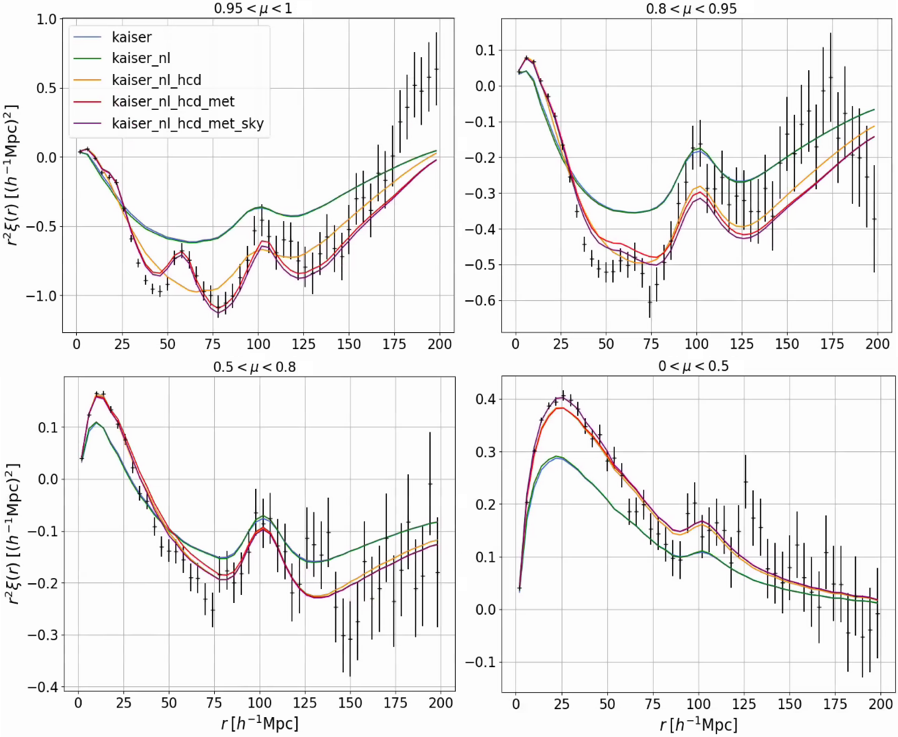
\includegraphics[scale=0.5]{cf_models}
  \caption{Les différentes composantes du modèle ajusté sur l'auto-corrélation \lya{}$\times$\lya{} des données DR16.
    La ligne bleue donne le modèle de Kaiser, c'est à dire la fonction de corrélation obtenue à partir du spectre de puissance $P_{\mathrm{QL}}$ (équation~\ref{eq:pk_ql}) multiplié par le facteur de Kaiser $b_{\mathrm{eff},\mathrm{Ly}\alpha}^2 (1 + \beta_{\mathrm{Ly}\alpha} \mu_k^2)$. La ligne verte donne le modèle de Kaiser multiplié par le terme $F_{\mathrm{NL}}^{\mathrm{auto}}$ qui prend en compte les non-linéarités aux petites échelles. La ligne orange donne le modèle précédent auquel la contribution des HCD a été ajoutée (équation~\ref{eq:bias_hcd_def}). La ligne rouge donne le modèle précédent plus la contribution des métaux et la ligne violette donne le modèle complet. L'auto-corrélation \lya{}$\times$\lya{} estimée à partir des données DR16 et moyennée dans les quatre bins en redshift est représentée par les points noirs.
Les quatre graphiques présentent 4 gammes en $\mu$ différentes.}
  \label{fig:cf_models}
\end{figure}
\begin{figure}
  \centering
  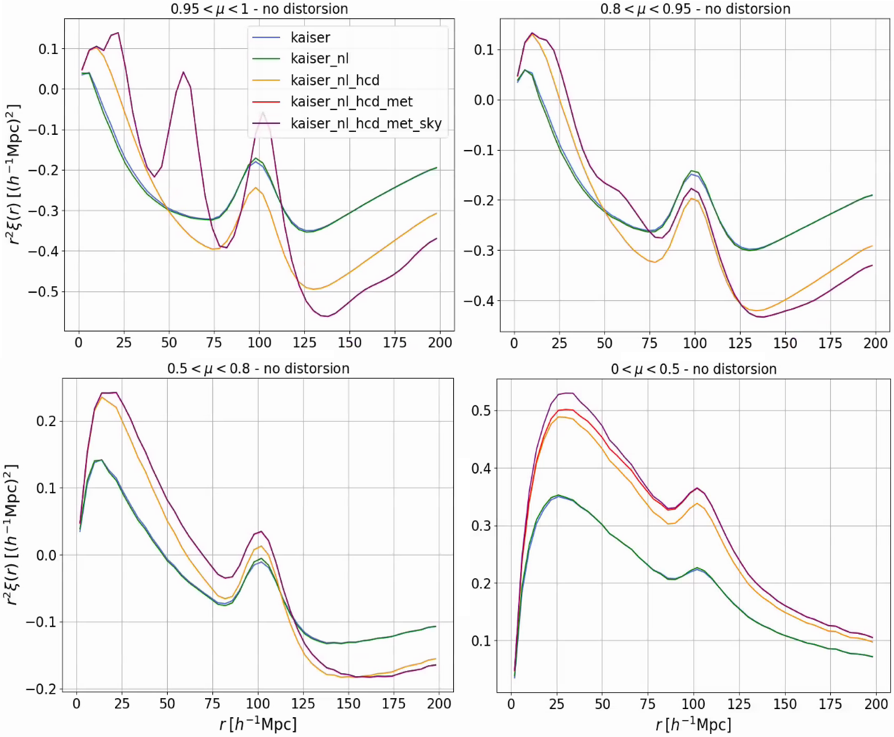
\includegraphics[scale=0.5]{cf_models_no_dist}
  \caption{Les différentes composantes du modèle ajusté sur l'auto-corrélation \lya{}$\times$\lya{} des données DR16. Elles sont décrites dans la légende de la figure~\ref{fig:cf_models}.
    Les composantes présentées ici n'incluent pas les distorsions produites par l'ajustement du continuum.
    Les quatre graphiques présentent ces composantes dans 4 gammes en $\mu$.}
  \label{fig:cf_models_no_dist}
\end{figure}



\subsubsection{Des HCD avec une même densité de colonne}
Nous avons ensuite regardé l'effet des différentes gammes de densité de colonne des HCD sur la fonction de corrélation \lya{}$\times$\lya{}.
Pour ce faire, à partir de la même réalisation des mocks, nous avons produit cinq versions eboss-0.2. Dans chacune de ces versions, nous ajoutons les HCD avec une densité de colonne fixe. Ces valeurs pour les cinq versions sont $\log n_{\mathrm{HI}} \in [\num{17.6}\,;\num{18.2}\,;\num{18.8}\,;\num{19.4}\,;\num{20}]$. Les nombres relatifs de HCD entre ces versions suivent la distribution en $\log n_{\mathrm{HI}}$ utilisée pour construire le catalogue standard de HCD (présentée sur la figure~\ref{fig:distrib_dla}). La distribution en $z$ utilisée est trois fois plus importante que dans le catalogue standard afin d'avoir suffisamment de HCD dans chaque gamme.

La figure~\ref{fig:cf_nhi_bins} présente les fonctions de corrélation \lya{}$\times$\lya{} pour les différentes versions des mocks décrites précédemment. Pour simplifier les comparaisons, nous n'utilisons pas de bins en redshift, les fonctions de corrélation sont donc estimées à partir de l'ensemble des forêts.
% La ligne bleue foncée donne la corrélation pour les mocks eboss-0.0 (sans HCD). La ligne violette donne la corrélation pour les mocks eboss-0.2 incluant les HCD avec $\num{17.2} < \log n_{\mathrm{HI}} < \num{20.3}$. Les autres couleurs donnent les corrélations pour les mocks eboss-0.2 incluant des HCD avec une valeur fixe en $\log n_{\mathrm{HI}}$.
Nous pouvons voir sur la figure~\ref{fig:cf_nhi_bins} que les HCD qui ont le plus grand effet sur la fonction de corrélation sont les HCD avec une grande densité de colonne, malgé leur nombre plus restreint. L'effet causé par les HCD avec une densité de colonne de \num{17.6}, \num{18.2} et \num{18.8} est similaire : la faible densité de colonne est compensée par le nombre plus important de HCD.

\begin{figure}
  \centering
  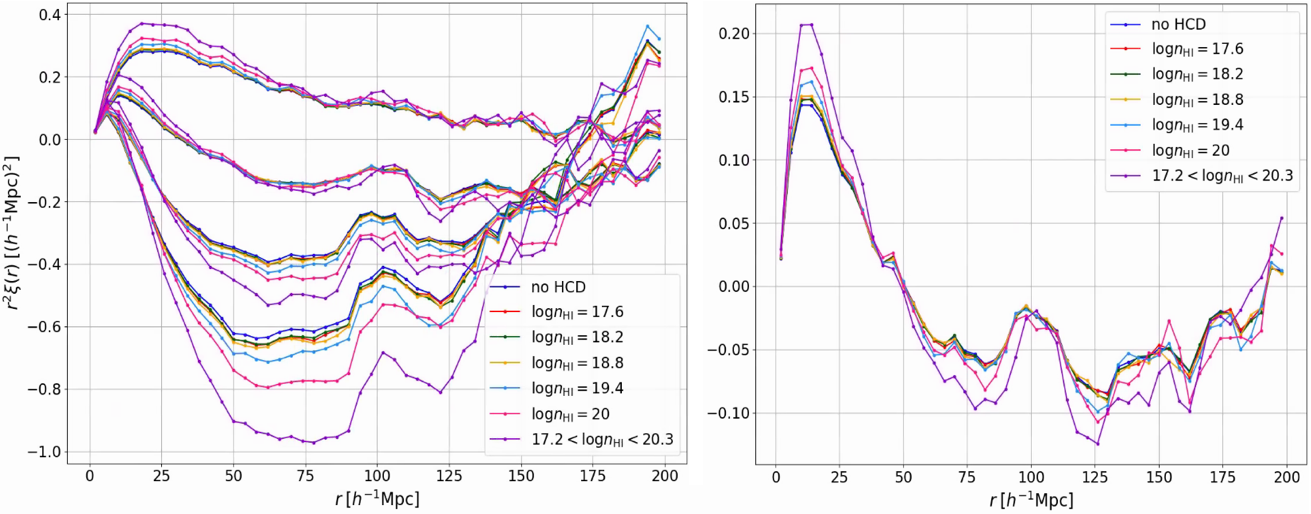
\includegraphics[scale=0.35]{cf_nhi_bins}
  \caption{Fonctions de corrélation \lya{}$\times$\lya{} estimées à partir d'une réalisation.
    La ligne bleue foncée donne la corrélation pour les mocks eboss-0.0 (sans HCD). La ligne violette donne la corrélation pour les mocks eboss-0.2 incluant les HCD avec $\num{17.2} < \log n_{\mathrm{HI}} < \num{20.3}$. Les autres couleurs donnent les corrélations pour les mocks eboss-0.2 incluant des HCD avec une valeur fixe en $\log n_{\mathrm{HI}}$.
    % Chaque couleur donne la densité de colonne $\log n_{\mathrm{HI}}$ utilisée pour générer les HCD. Le détail est donné dans le texte.
    Le graphique de gauche montre les corrélations dans quatre gammes en $\mu$. Ces gammes sont, de haut en bas : $\num{0}<\mu<\num{0.5}$, $\num{0.5}<\mu<\num{0.8}$, $\num{0.8}<\mu<\num{0.95}$ et $\num{0.95}<\mu<\num{1}$. Le graphique de droite montre les corrélations moyennées sur $\num{0} < \mu < \num{1}$.}
  \label{fig:cf_nhi_bins}
\end{figure}

\paragraph{}
Afin de comprendre les différences entre le modèle de Rogers et le modèle C-G observées sur la figure~\ref{fig:bias_cg_rogers_comp},
nous étudions maintenant comment ces deux modèles se comportent lorsque nous ajustons les mocks contenant des HCD avec une densité de colonne fixe.
Dans chacun des ajustements, nous devons utiliser pour chaque modèle un terme $F_{\textsc{HCD}}$ adéquat aux HCD présents.
En ce qui concerne le modèle de C-G, le code \texttt{picca} permet de calculer le terme $F_{\textsc{HCD}}$ pour une distribution en $\log n_{\mathrm{HI}}$ données. Nous calculons donc $F_{\textsc{HCD}}$ pour chacune des valeurs de $\log n_{\mathrm{HI}}$.
Pour le modèle de Rogers, la forme de $F_{\textsc{HCD}}$ est fixée (équation~\ref{eq:f_hcd_def}). Il nous suffit, pour chaque valeur de $\log n_{\mathrm{HI}}$, de trouver la valeur de $L_{\textsc{HCD}}$ à utiliser. Mais ceci n'est pas chose aisée. Dans l'analyse DR16, $L_{\textsc{HCD}}$ est choisie de manière un peu arbitraire à \SI{10}{\perh\Mpc}, car il influence très peu la mesure des paramètres BAO.
Mais comme nous l'avons vu à plusieurs reprises, $L_{\textsc{HCD}}$ influence grandement la mesure des paramètres \lya{}. Nous devons donc le choisir avec précaution.

\begin{figure}
  \centering
  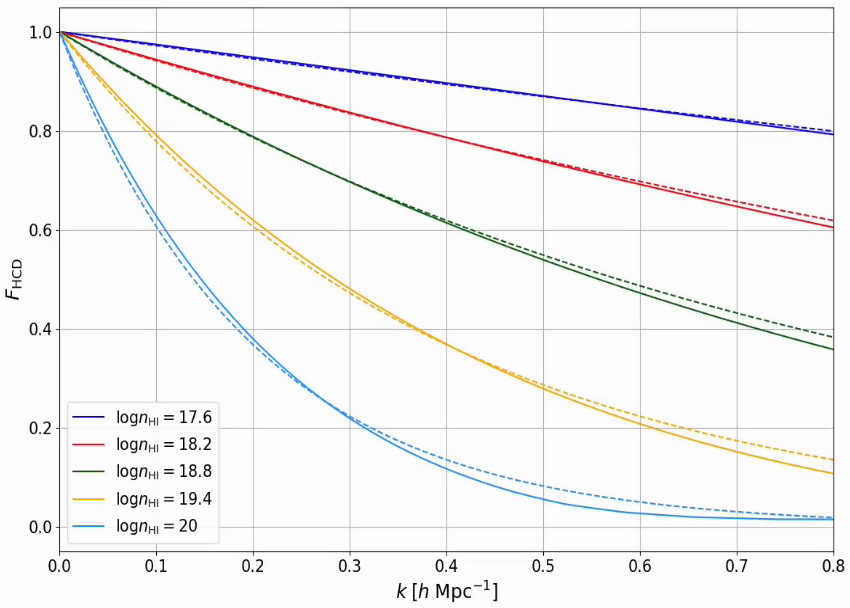
\includegraphics[scale=0.4]{f_hcd_fixed}
  \caption{Les fonctions $F_{\textsc{HCD}}$ utilisées dans le cadre du modèle C-G (lignes continues) ou du modèle de Rogers (lignes tiretées) pour différentes valeurs de $\log n_{\mathrm{HI}}$. Les valeurs de  $L_{\textsc{HCD}}$ utilisées pour le modèle de Rogers sont données dans le texte.
}
  \label{fig:f_hcd_fixed}
\end{figure}

% Nous déterminons $L_{\textsc{HCD}}$ de deux façons différentes.
Nous expliquons ici la méthode utilisée pour déterminer $L_{\textsc{HCD}}$.
Pour chaque valeur de $\log n_{\mathrm{HI}}$, nous choisissons une valeur de $L_{\textsc{HCD}}$ qui reproduise au mieux le comportement de $F_{\textsc{HCD}}(k)$ calculé dans le modèle C-G dans la gamme $k \lesssim \SI{0.8}{\h\per\Mpc}$. % c'est à dire pour des échelles supérieures à $r \sim \SI{10}{\perh\Mpc}$.
Nous ne nous intéressons pas aux $k$ plus grands que \SI{0.8}{\h\per\Mpc} car la fonction de corrélation est estimée dans des bins de \SI{4}{\perh\Mpc}, les échelles plus petites que $k = \pi / 4 \sim \SI{0.8}{\h\per\Mpc}$ ne sont donc pas accessibles.
Ainsi, les valeurs de $L_{\textsc{HCD}}$ que nous obtenons pour $\log n_{\mathrm{HI}} \in [\num{17.6}\,;\num{18.2}\,;\num{18.8}\,;\num{19.4}\,;\num{20}]$ sont $L_{\textsc{HCD}} \in [\num{0.28}\,; \num{0.60}\,; \num{1.2}\,; \num{2.5}\,; \num{5}]$.
% Ainsi, afin de reproduire le comportement de $F_{\textsc{HCD}}(k)$ pour $k \lesssim \SI{0.8}{\h\per\Mpc}$, les valeurs de $L_{\textsc{HCD}}$ que nous choisissons pour $\log n_{\mathrm{HI}} \in [\num{17.6}\,;\num{18.2}\,;\num{18.8}\,;\num{19.4}\,;\num{20}]$ sont $[\num{0.28}\,; \num{0.60}\,; \num{1.2}\,; \num{2.5}\,; \num{5}]$.
La figure~\ref{fig:f_hcd_fixed} présente les fonctions $F_{\textsc{HCD}}(k)$ pour le modèle C-G (lignes continues) et pour le modèle de Rogers (lignes tiretées) en utilisant les valeurs de $L_{\textsc{HCD}}$ obtenues précédemment.
% Les lignes continues donnent les fonctions $F_{\textsc{HCD}}(k)$ calculées par \texttt{picca}. Ce sont les fonctions utilisées dans le cadre du modèle de C-G. Les lignes tiretées donnent les termes $F_{\textsc{HCD}}(k)$ pour le modèle de Rogers, c'est à dire $F_{\textsc{HCD}}(k) = \exp(- L_{\textsc{HCD}} k)$.
Pour chaque valeur de $\log n_{\mathrm{HI}}$, les fonctions $F_{\textsc{HCD}}$ sont très similaires entre les deux modèles.

Nous ajustons maintenant chacune des versions des mocks avec les deux modèles. Pour le modèle de Rogers, nous utilisons les valeurs de $L_{\textsc{HCD}}$ déterminées précédemment.
Pour chacune des versions des mocks, les ajustements faits avec le modèle de Rogers et le modèle C-G produisent des résultats très similaires. Les différences sont inférieures au dizième de $\sigma$.
Ceci est rassurant car les fonctions $F_{\textsc{HCD}}$ utilisées dans ces deux modèles sont très similaires.
Par ailleurs, pour les faibles valeurs de $\log n_{\mathrm{HI}}$, les fonctions $F_{\textsc{HCD}}$ sont très proches de 1 (figure~\ref{fig:f_hcd_fixed}). Les paramètres \lya{} et HCD sont alors quasiment complètement dégénérés. Le paramètre $\beta_{\mathrm{Ly}\alpha}$, en particulier, n'est pas contraint.  Lorsque $\log n_{\mathrm{HI}}$ est plus grand (supérieur à \num{18.8}), les ajustements parviennent à mesurer les paramètres du \lya{}.
Cependant ces mesures ne sont pas compatibles entre elles et ne sont pas non plus compatibles avec les mesures faites sur les mocks eboss-0.0.
Si ces modèles ne parviennent pas à distinguer l'effet du \lya{} de l'effet des HCD lorsque ces derniers possèdent une densité de colonne fixe, alors il y a peu d'espoirs qu'ils parviennent à le faire lorsque les HCD sont distribués dans une large gamme en densité de colonne.

\paragraph{}
Nous comparons maintenant les fonctions $F_{\textsc{HCD}}$ correspondant à une large gamme en densité de colonne.
Nous considérons premièrement la gamme en densité de colonne des HCD présents dans les mocks eboss-0.2 lorsque les HCD avec $\log n_{\mathrm{HI}} > \num{20.3}$ sont masqués, c'est à dire la gamme $\num{17.2} < \log n_{\mathrm{HI}} < \num{20.3}$. 
La fonction $F_{\textsc{HCD}}$ utilisée dans le modèle de C-G pour cette gamme en $\log n_{\mathrm{HI}}$ est calculée par \texttt{picca}.
Comme précédemment, afin de déterminer le $L_{\textsc{HCD}}$ à utiliser dans le modèle de Rogers, nous cherchons à reproduire le comportement de $F_{\textsc{HCD}}(k)$ utilisé dans le modèle de C-G dans la gamme $k \lesssim \SI{0.8}{\h\per\Mpc}$. Pour ce faire, nous devons choisir $L_{\textsc{HCD}} = \SI{2.8}{\perh\Mpc}$.
La figure~\ref{fig:f_hcd_range} présente les fonctions $F_{\textsc{HCD}}$ ainsi obtenues (en bleu). Nous pouvons remarquer que pour une large gamme en $\log n_{\mathrm{HI}}$, il est plus difficile d'obtenir un accord entre le modèle de Rogers et le modèle C-G.
La figure~\ref{fig:f_hcd_range} présente aussi, à titre de comparaison, la  fonction $F_{\textsc{HCD}}$ obtenue avec $L_{\textsc{HCD}} = \SI{10}{\perh\Mpc}$ (en vert).
La différence entre la courbe continue bleue et la courbe tiretée verte est très importante. Nous sommes étonnés\footnote{Nous pensons que cela vient du biais des HCD qui est environ \num{2.2} fois supérieur dans la mesure faite avec le modèle C-G. Nous pensons que le biais des HCD plus faible obtenu avec le modèle de Rogers compense les mesures des paramètres \lya{}.} que les ajustements faits sur les mocks eboss-0.2 avec le modèle de Rogers (avec $L_{\textsc{HCD}} = \SI{10}{\perh\Mpc}$) et le modèle C-G produisent des résultats si similaires (respectivement en rose et en jaune sur la figure~\ref{fig:bias_cg_rogers_comp}) compte tenu de ces différences sur $F_{\textsc{HCD}}$.
  Dans tous les cas, nous pensons que la mesure faite avec $L_{\textsc{HCD}} = \SI{10}{\perh\Mpc}$ n'est pas fiable.
La figure~\ref{fig:f_hcd_range} présente aussi, en rouge, les fonctions $F_{\textsc{HCD}}$ obtenues pour la gamme $\num{17.2} < \log n_{\mathrm{HI}} < \num{22.5}$. La valeur de $L_{\textsc{HCD}}$ choisie est \SI{6.5}{\perh\Mpc}. Les fonctions $F_{\textsc{HCD}}$ obtenues pour cette gamme dans le cadre du modèle C-G et du modèle de Rogers (courbes rouges) sont très différentes. Le modèle de Rogers atteint ici ses limites.


\begin{figure}
  \centering
  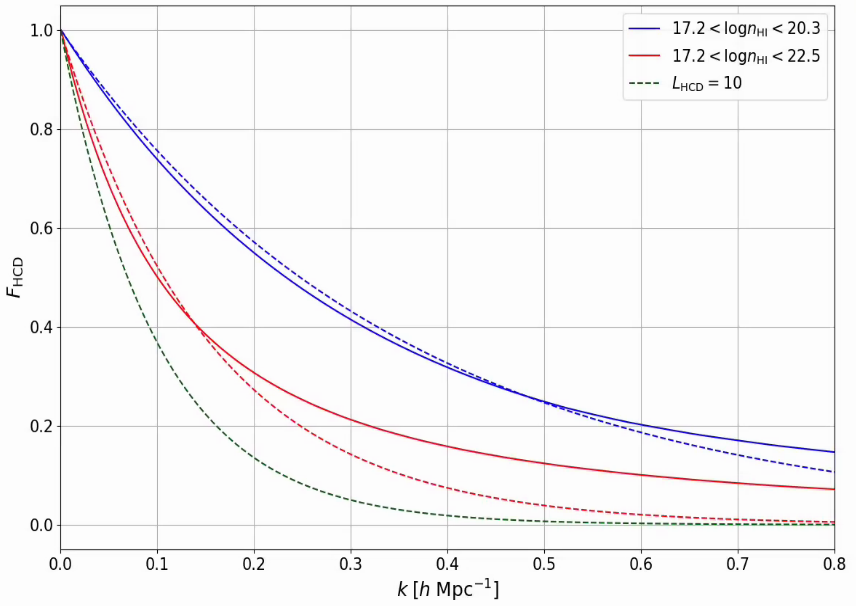
\includegraphics[scale=0.4]{f_hcd_range}
  \caption{Les fonctions $F_{\textsc{HCD}}$ utilisées dans le cadre du modèle C-G (lignes continues) ou du modèle de Rogers (lignes tiretées).
    Les courbes bleues correspondent à la gamme $\num{17.2} < \log n_{\mathrm{HI}} < \num{20.3}$. Les courbes rouges correspondent à la gamme $\num{17.2} < \log n_{\mathrm{HI}} < \num{22.5}$. La courbe verte donne $F_{\textsc{HCD}}$ utilisé dans le modèle de Rogers avec $L_{\textsc{HCD}} = \SI{10}{\perh\Mpc}$.
}
  \label{fig:f_hcd_range}
\end{figure}

\paragraph{}
Suite à ces observations, nous reproduisons l'analyse des mocks eboss-0.2 où les HCD avec une densité de colonne $\log n_{\mathrm{HI}} > \num{20.3}$ sont masqués. Nous analysons les fonctions de corrélation \lya{}$\times$\lya{} en utilisant le modèle de Rogers, avec $L_{\textsc{HCD}} = \SI{2.8}{\perh\Mpc}$. Ainsi, nous vérifions que les résultats de l'ajustement sont très similaires à ceux obtenus avec le modèle C-G (les résultats varient d'un dixième de $\sigma$). Ceci est attendu car les fonctions $F_{\textsc{HCD}}$ sont très similaires.
De plus, comme nous l'avons vu dans la section~\ref{subsec:model_alter_hcd}, la mesure des paramètres \lya{} faite sur les mocks eboss-0.2 où les HCD avec une densité de colonne $\log n_{\mathrm{HI}} > \num{20.3}$ sont masqués et ajustés avec le modèle C-G, est compatible avec la mesure faite sur les mocks eboss-0.2 où aucun HCD n'est masqué et ajustés avec le modèle C-G. Ainsi les trois mesures des paramètres \lya{} que nous faisons (modèle C-G avec ou sans HCD masqués et modèle de Rogers avec $L_{\textsc{HCD}} = \SI{2.8}{\perh\Mpc}$) sur les mocks eboss-0.2 sont compatibles.
Cependant il reste toujours un léger écart entre la mesure faite sur les mocks eboss-0.0 et celle faite sur les mocks eboss-0.2 (environ \SI{5}{\percent}, voir figure~\ref{fig:bias_cg_rogers_comp}).

\begin{figure}
  \centering
  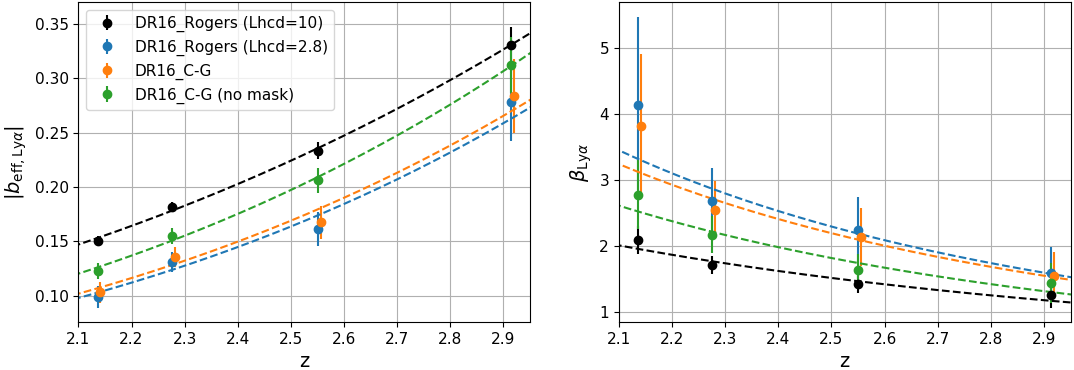
\includegraphics[scale=0.44]{bias_dr16_comp}
  \caption{Mesure des paramètres $b_{\mathrm{eff},\mathrm{Ly}\alpha}$ (gauche) et $\beta_{\mathrm{Ly}\alpha}$ (droite) sur l'auto-corrélation \lya$\times$\lya{} estimée à partir des données DR16. Les points bleus présentent la mesure faite avec le modèle de Rogers en utilisant $L_{\textsc{HCD}} = \SI{2.8}{\perh\Mpc}$. Les points orange la mesure faite avec le modèle C-G lorsque les HCD avec $\log n_{\mathrm{HI}} > \num{20.3}$ sont masqués. Les points verts la mesure faite avec le modèle C-G lorsqu'aucun HCD n'est masqué. Enfin, les points noirs présentent la mesure faite avec le modèle de Rogers en utilisant $L_{\textsc{HCD}} = \SI{10}{\perh\Mpc}$.
      Les courbes tiretées correspondent à l'ajustement de chaque jeu de données par une loi de puissance.
Les points orange sont décalés horizontalement de $\Delta z = 5\times10^{-3}$ pour des raisons de visibilité.}
  \label{fig:bias_dr16_comp}
\end{figure}

\paragraph{}
Après avoir fait ces vérifications sur les mocks, nous analysons les données DR16 avec les modèles de HCD étudiés précédemment. La figure~\ref{fig:bias_dr16_comp} présente les mesures des paramètres \lya{} faites sur les données DR16 en utilisant ces différents modèles de HCD.
Nous pouvons premièrement remarquer que, comme pour les mocks, la mesure faite avec le modèle C-G lorsque les HCD avec une densité de colonne $\log n_{\mathrm{HI}} > \num{20.3}$ sont masqués (orange) est très similaires à la mesure faite avec le modèle de Rogers lorsque nous utilisons $L_{\textsc{HCD}} = \SI{2.8}{\perh\Mpc}$ (bleu). Cependant, contrairement aux mocks, ces deux mesures ne sont pas compatibles avec la mesure faite avec le modèle C-G lorsqu'aucun HCD n'est masqué (vert).
% A titre de comparaison, la mesure faite avec le modèle de Rogers avec $L_{\textsc{HCD}} = \SI{10}{\perh\Mpc}$ (utilisée comme référence pour construire les mocks) est montrée en noir.
Le fait que les deux mesures faites avec le modèle C-G (HCD masqués ou non) ne soient pas compatibles, alors que les mêmes mesures faites sur les mocks le sont (voir figure~\ref{fig:bias_cg_rogers_comp}), pose un sérieux problème. Cela signifie que quelque chose dans les données ne se comporte pas de la même manière que dans les mocks. Il se pourrait qu'un effet inconnu, présent dans les données, soit pris en compte par la modélisation des HCD. Cependant nous n'avons pour l'instant pas d'intuition concernant la nature de cet effet.


\paragraph{}
La dernière analyse que nous effectuons est d'étudier comment se comporte la valeur de $\chi^2$ de l'ajustement en fonction du paramètre $L_{\textsc{HCD}}$. Nous effectuons cette étude à la fois pour les mocks et pour les données.
La figure~\ref{fig:L0_free} présente la valeur de $\chi^2$ de l'ajustement obtenue pour différentes valeurs de $L_{\textsc{HCD}}$.
% Le graphique de gauche présente les mesures faites sur les mocks eboss-0.2, où les HCD avec une densité de colonne $\log n_{\mathrm{HI}} > \num{20.3}$ sont masqués. Le graphique de droite présente les mesures faites sur les données DR16, où les HCD sont aussi masqués. Sur ces deux graphiques, le point rouge présente la mesure, ainsi que la barre d'erreur qui l'accompagne, du paramètre $L_{\textsc{HCD}}$ lorsqu'il est laissé libre dans l'ajustement.
Sur les données DR16 (graphique de droite), nous mesurons $L_{\textsc{HCD}} = \num{2.54} \pm \num{0.73} \si{\perh\Mpc}$, ce qui est en accord avec la valeur suggérée par l'analyse présentée dans les paragraphes précédents.
Cependant, lorsque nous faisons le même exercice sur les mocks (graphique de gauche), nous mesurons $L_{\textsc{HCD}} = \num{11.73} \pm \num{4.75} \si{\perh\Mpc}$. Cette mesure est peu contrainte sur les mocks, et en tension ($\sim 2 \sigma$) avec la valeur $L_{\textsc{HCD}} = \num{2.8} \si{\perh\Mpc}$ suggérée par les analyses présentées précédemment.

\begin{figure}
  \centering
  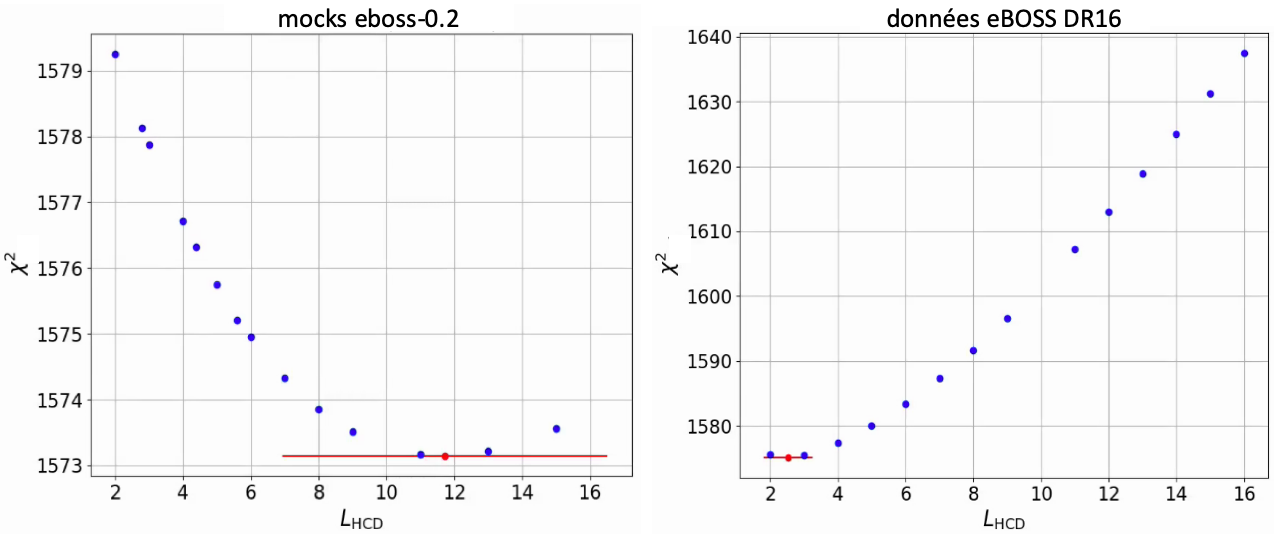
\includegraphics[scale=0.36]{L0_free}
  \caption{Evolution de la valeur de $\chi^2$ de l'ajustement en fonction du paramètre $L_{\textsc{HCD}}$. La figure de gauche montre l'évolution pour les mocks eboss-0.2 où les HCD avec une densité de colonne $\log n_{\mathrm{HI}} > \num{20.3}$ sont masqués. Celle de droite l'évolution pour les données DR16 où les HCD sont aussi masqués. Sur chaque graphique, le point rouge présente la valeur, ainsi que la barre d'erreur qui l'accompagne, de $L_{\textsc{HCD}}$ qui minimise le $\chi^2$.}
  \label{fig:L0_free}
\end{figure}

Ici encore, nous sommes face à une incohérence : lorsque nous étudions la distribution des HCD présents dans les mocks (avec une densité de colonne comprise dans la gamme $\num{17.2} < \log n_{\mathrm{HI}} < \num{20.3}$), le modèle C-G nous suggère d'utiliser $L_{\textsc{HCD}} = \SI{2.8}{\perh\Mpc}$. Pourtant lorsque $L_{\textsc{HCD}}$ est laissé libre, la valeur obtenue est en tension avec $L_{\textsc{HCD}} = \num{2.8} \si{\perh\Mpc}$.
Quand nous fixons les paramètres \lya{} aux valeurs mesurées sur les mocks eboss-0.0 et laissons libre $L_{\textsc{HCD}}$, nous mesurons $L_{\textsc{HCD}} = \num{4.38} \pm \num{0.47} \si{\perh\Mpc}$. Ceci a pour effet de réduire les tensions. Mais la mesure produite n'est tout de même pas compatible ($\sim 3 \sigma$) avec ce que suggère le modèle C-G.


\paragraph{}
Après ces nombreuses études, nous ne sommes pas convaincus quant au modèle de HCD à utiliser pour ajuster les données.
Le fait que la mesure du paramètre $L_{\textsc{HCD}}$, quand il est laissé libre, soit compatible avec ce que suggère le modèle C-G (grâce à l'étude des fonctions $F_{\textsc{HCD}}$) encourage à utiliser le modèle de Rogers avec $L_{\textsc{HCD}} = \SI{2.8}{\perh\Mpc}$, où de manière équivalente le modèle C-G lorsque les HCD avec une densité de colonne $\log n_{\mathrm{HI}} > \num{20.3}$ sont masqués.
Cependant, le fait que ce résultat ne soit pas également obtenu sur les mocks, c'est à dire que la valeur du paramètre $L_{\textsc{HCD}}$ obtenu lorsqu'il est laissé libre dans l'ajustement des mocks eboss-0.2 (avec les HCD masqués) ne soit pas compatible avec la valeur suggérée par l'étude des fonctions $F_{\textsc{HCD}}$ avec le modèle C-G, ne nous encourage pas à utiliser le modèle de Rogers avec $L_{\textsc{HCD}} = \SI{2.8}{\perh\Mpc}$.

De plus, le fait que les ajustements effectués sur les données DR16 avec le modèle C-G, lorsque les HCD sont masqués ou ne sont pas masqués, ne soient pas compatibles ne nous conforte pas dans l'idée d'utiliser aveuglément ce modèle.
Il est probable que des effets systématiques inconnus soient présents dans les données, et que les différents modèles de HCD prennent ces effets en compte.

Etant donné l'état de connaissance actuel de la modélisation des HCD et des effets systématiques qui pourraient affecter les données, nous pensons qu'il est préférable d'utiliser le modèle C-G sans masquer les HCD dans les données.
Premièrement, le fait de ne pas masquer les HCD permet d'avoir plus de pixel d'absorptions dans l'analyse, et donc de disposer de plus de statistique pour effectuer la mesure de la position du pic BAO.
De plus, lorsque le nombre de HCD présents dans les données est plus important, la fonction $F_{\textsc{HCD}}$ est plus importante est donc les paramètres \lya{} et ceux des HCD sont moins corrélés.
Deuxièmement, le fait de masquer les HCD consiste à retirer une partie non aléatoire des données, qui plus est qui correspond à des régions denses de l'univers.
Un tel processus peut introduire des effets systématiques dans l'analyse.
Pour ces raisons, nous pensons qu'il est préférable de ne pas masquer les HCD, et donc d'utiliser le modèle C-G.



% \printbibliography
% \end{document}
